\documentclass[11pt,a4paper]{report}
%%%%%%%%%%%%%%%%%%%%%%%%%%%%%%%%%%%%%%%%%%%%%%%%%%%%%%%%%%%%%%%%%%%%%
%%                                                                 %%
%%    Header file for the Phi-S-X Series                           %%
%%                                                                 %%
%%    german version header_gm.tex is derived from header.tex      %%
%%    by uncommenting the line ``\setboolean{german}{true}'' below %%
%%                                                                 %%
%%    Never edit the german version! all changes must be done      %%
%%    in the english version header.tex                            %%
%%                                                                 %%
%%%%%%%%%%%%%%%%%%%%%%%%%%%%%%%%%%%%%%%%%%%%%%%%%%%%%%%%%%%%%%%%%%%%%
%%%%%%%%%%%%%%%%%%%%%%%%%%%%%%%%%%%%%%%%%%%%%%%%%%%%%%%%%%%%%%%%%%%%%
%%                                                                 %%
%%    Header file for the Phi-S-X Series                           %%
%%                                                                 %%
%%    german version header_gm.tex is derived from header.tex      %%
%%    by uncommenting the line ``\setboolean{german}{true}'' below %%
%%                                                                 %%
%%    Never edit the german version! all changes must be done      %%
%%    in the english version header.tex                            %%
%%                                                                 %%
%%%%%%%%%%%%%%%%%%%%%%%%%%%%%%%%%%%%%%%%%%%%%%%%%%%%%%%%%%%%%%%%%%%%%
%====================================================================
%-- define flag for language adaptations
\usepackage{ifthen}   % allows to select only certain text
\provideboolean{german}
\setboolean{german}{false}
%\setboolean{german}{true}  % uncomment this line for german editions
%====================================================================
%
% Textschriftart: Computer modern Bright
% body:            CM-Bright 10pt
% section titles:  CM-Bright Bold
% formulas:        CM-Bright Math Oblique
%
\usepackage[standard-baselineskips]{cmbright}
\usepackage{cmbright}
\usepackage[T1]{fontenc}
\def\usedfonts{CM-Bright}
\usepackage{typearea}
%\typearea[current]{calc} % benutzt die aktuelle 
       % bindekorrektur (BCOR angabe als parameter in koma usepackage)
       % und berechnet satzspiegel neu
\typearea[current]{11} %fixed div value

\usepackage{textcomp} % special symbols
\usepackage{amsfonts} % special symols
                      % see ftp://ftp.ams.org/pub/tex/doc/amsfonts/amsfndoc.pdf
\usepackage{amssymb}  % CM-Bright provides the AMS symbols
\usepackage{exscale}  % allows to scale math expressions to big fonts, 
                      % e.g. \Huge
\usepackage{curves}
\usepackage{braket}
\usepackage{miller}     % miller indices
\usepackage{chemmacros} % http://www.mychemistry.eu/mychemistry/
\usepackage[numbers]{natbib}     % bibliography style
\usepackage{url}\urlstyle{tt}
\usepackage{float}
\usepackage{bm}       % provides the command \bm{} that makes bold math symbols
\usepackage{amsmath}
\usepackage{amsbsy}   % allows bold mathematical symbols
\usepackage{amscd}
 \usepackage{a4wide}  % it is better to use the ``geometry'' package
\usepackage{array}    % 
\usepackage{fancyhdr} %  defines pagestyle fancy
\usepackage{epsfig}   % include graphics with epsfig
\usepackage{graphicx} % includegraphics
\usepackage{epstopdf}
\usepackage{wrapfig}
\usepackage{fancybox} % allows shadow-boxes
\usepackage{color}    % allows to use color in the text
%\usepackage{eepic}
\usepackage{flafter}  % places picture next to its reference
\usepackage{makeidx}  % make an index
%\usepackage{MnSymbol}  % 
%\usepackage{marvosym}  % 
\usepackage{textcase}
\usepackage{ulem} % defines strikeout \sout{}; underline \uline{}
                  % double underline \uuline{}; wave underline \uwave{}
                  % cross out \xout{}
%
%==========================================================================
%==  page layout  =========================================================
%==========================================================================
% eqnarray environment: reduce with of space in place of each ``&''
\setlength\arraycolsep{1.4pt}
\pagestyle{fancy}
%\renewcommand{\chaptermark}[1]{\markboth{\thechapter\ #1}{}}
\renewcommand{\chaptermark}[1]{\markboth{\MakeUppercase{\thechapter\ #1}}{}}
\fancyhf{} 
\fancyhead[LE]{\textsc{\thepage}\qquad\textsc{\leftmark}}
\fancyhead[RO]{\textsc{\leftmark}\qquad\textsc{\thepage}}
\renewcommand{\headrulewidth}{0.5pt}
\renewcommand{\footrulewidth}{0pt} 
\addtolength{\headheight}{2.5pt}
\fancypagestyle{plain}{\fancyhead{}
   \renewcommand{\headrulewidth}{0pt}
   \fancyfoot[CO]{\bfseries\thepage}}

% Line spacing -----------------------------------------------------------
\newlength{\defbaselineskip}
\setlength{\defbaselineskip}{\baselineskip}
\newcommand{\setlinespacing}[1]%
           {\setlength{\baselineskip}{#1 \defbaselineskip}}
\newcommand{\doublespacing}{\setlength{\baselineskip}%
                           {2.0 \defbaselineskip}}
\newcommand{\singlespacing}{\setlength{\baselineskip}{\defbaselineskip}}

% Absatz einr\"ucken ------------------------------------------------------
%\setlength{\parindent}{0pt}
\setlength{\parskip}{2pt}
% -------------------------------------------------------------------------
\ifthenelse{\boolean{german}}
  {\def\figurename{Abb.}}
  {\def\figurename{Fig.}}
%--------------------------------------------------------------------------
\renewcommand{\arraystretch}{1.15}  % skaliert den Zeilen abstand in der 
    % tabular und array umgebung
%
%==========================================================================
%==  boxes etc ============================================================
%==========================================================================
%== minipage in a shadowbox ===============================================
\newenvironment{myshadowminipage}[1]%
  {\par\noindent\begin{Sbox}\begin{minipage}{\linewidth}\vspace{0.1cm}\begin{center}\uppercase{#1}\end{center}}%
  {\vspace{0.1cm}\end{minipage}\end{Sbox}\shadowbox{\TheSbox}}
%
%== minipage in a framedbox ===============================================
\newenvironment{myframedminipage}%
  {\par\noindent\begin{Sbox}\begin{minipage}\linewidth\vspace{0.1cm}}%
  {\vspace{0.1cm}\end{minipage}\end{Sbox}\fbox{\TheSbox}}
%
\newcommand{\myshadowbox}[1]{\noindent\shadowbox{\parbox{\linewidth}{\smallskip #1\smallskip}}}
\newcommand{\myfbox}[1]{\noindent\fbox{\parbox{\linewidth}{\smallskip #1\smallskip}}\medskip}
%== minipage in a framedbox ===============================================
\newtheorem{defi}{Definition}[chapter]
\newenvironment{definition}[1]%
  {\par\noindent\begin{Sbox}\begin{minipage}{\linewidth}\vspace{0.1cm}\begin{defi}\uppercase{#1}\\\vspace{0.1cm}}%
  {\vspace{0.1cm}\end{defi}\end{minipage}\end{Sbox}\shadowbox{\TheSbox}}
%
%=========================================================================
% color used to point out information to the teacher
\definecolor{highlight}{rgb}{1.0,0.7,0.}
\newcommand{\Special}[1]{\textbf{\textcolor{highlight}{#1}}}
%=========================================================================
%  switch certain parts on and off. uses ifthen package
\newboolean{teacher}\setboolean{teacher}{false}
% this parameter can be changed in the manuscript again
\setboolean{teacher}{true} %private version if true!
\newcommand{\teacheronly}[1]{\ifthenelse{\boolean{teacher}}{#1\hfill\\ }}
\newcommand{\editor}[1]{\textcolor{blue}{\texttt{Editor: #1}}}
\newcommand{\MARK}[1]{\textcolor{blue}{#1}} 
\newcommand{\RED}[1]{\textcolor{red}{#1}} 
%
%==========================================================================
%==  define new symbols                                                 ===
%==========================================================================
% define \stat (stationary state) as an operator like \min
\DeclareMathOperator*{\stat}{stat}
\let\Vec=\mathbold   % cmbright.sty provides a bold/italic math alphabet
\let\Dot=\mathbold   % cmbright.sty provides a bold/italic math alphabet
\let\Ddot=\mathbold   % cmbright.sty provides a bold/italic math alphabet
%
\newcommand{\e}[1]{\mathrm{e}^{#1}}% exponential function
\renewcommand{\Re}{\mathrm{Re}}    % real part
\renewcommand{\Im}{\mathrm{Im}}    % imaginary part
\newcommand{\lagr}{\ell}           % Lagrange dichte
\newcommand{\Lagr}{\mathcal{L}}    % Lagrange Funktion
\newcommand{\erf}{{\rm erf}}       %
\newcommand{\atan}{{\rm atan}}     % arcus tangens
\newcommand{\mat}[1]{\bm{#1}}  % Matrix
\newcommand{\gmat}[1]{{\boldsymbol #1}}  % Matrix(symbol)
\newcommand{\defas}{\stackrel{\text{def}}{=}}  %  is defined as
\ifthenelse{\boolean{german}}
  {\newcommand{\rot}{{\rm\bf rot}}}    % curl
  {\newcommand{\rot}{{\rm\bf curl}}}   % curl
\newcommand{\sgn}{{\rm sgn}}       % sign
\ifthenelse{\boolean{german}}
   {\newcommand{\Tr}{\mathrm{Sp}}}      % trace
   {\newcommand{\Tr}{\mathrm{Tr}}}      % trace
\ifthenelse{\boolean{german}}
   {\newcommand{\grmn}[2]{\footnote{``#2'' hei{\ss}t in englisch ``#1''}}}
   {\newcommand{\grmn}[2]{\footnote{``#1'' translates as ``#2'' into German}}}
% define the equation reference
\ifthenelse{\boolean{german}}
   {\newcommand{\eq}[1]{\text{Gl.}~\ref{#1}}}
   {\newcommand{\eq}[1]{\text{Eq.}~\ref{#1}}}
% define a relation with an equation number ontop
\newcommand{\eqrel}[2]{\stackrel{\eq{#1}}{#2}}
\newcommand{\zero}{\varnothing}
%\newcommand{\ket}[1]{|#1\rangle} % contained in package braket
\newcommand{\sumint}{\int\hspace{-15pt}\sum}
\newcommand{\marker}[1]{\textcolor{blue}{\emph{#1}}}
\renewcommand*{\dot}[1]{\overset{\mbox{\large\bfseries .}}{#1}}
\renewcommand*{\ddot}[1]{\overset{\mbox{\large\bfseries\hspace{+0.1ex}.\hspace{-0.1ex}.}}{#1}}
%
%==========================================================================
%==                                                                     ===
%==========================================================================
% Prevent figures from appearing on a page by themselves
% from http://dcwww.camd.dtu.dk/~schiotz/comp/LatexTips/LatexTips.html
\renewcommand{\topfraction}{0.85}
\renewcommand{\textfraction}{0.1}
\renewcommand{\floatpagefraction}{0.75}
%
%==========================================================================
%==                                                                     ===
%==========================================================================
\makeindex    % make index. uses makeidx package.

%== allow links between documents ============================================
\usepackage{xr}
\usepackage{xr-hyper}
%==  hyperref package (must be last package)
\usepackage[colorlinks=true]{hyperref} %specify this as last package
\hypersetup{citecolor=blue}
\hypersetup{menucolor=magenta}
\hypersetup{urlcolor=blue}      % 
\hypersetup{filecolor=green}    % file links
\hypersetup{linkcolor=magenta}  %table of contents
\hypersetup{pdfauthor={Peter E. Bl\"ochl}}
\hypersetup{pdfdisplaydoctitle=true}
\externaldocument[phisx1-]{/Users/ptpb/Tree/PhiSX/ClassicalMechanics/Book/cm-gm}
\externaldocument[phisx2-]{/Users/ptpb/Tree/PhiSX/Electrodynamics/Book/el-gm}
\externaldocument[phisx3-]{/Users/ptpb/Tree/PhiSX/QuantumMechanics/Book/qm}
\externaldocument[phisx4-]{/Users/ptpb/Tree/PhiSX/StatisticalMechanics/Book/sm}
\externaldocument[phisxqm2-]{/Users/ptpb/Tree/PhiSX/QuantumMechanicsII/Book/qm2}
\externaldocument[phisxsm2-]{/Users/ptpb/Tree/PhiSX/StatisticalMechanicsII/Book/sm2}
\externaldocument[phisxcb-]{/Users/ptpb/Tree/PhiSX/Chemicalbond/Book/cb}
% Example: Figure~PhiSX:Quantum
% Mechanics-\ref{phisx3-fig:doubleslitwave} on page
% \pageref{phisx3-fig:doubleslitwave}


\hypersetup{pdftitle=paw_brillouin}
\newcommand{\petertt}[1]{\textcolor{red}{\texttt{#1}}}
\begin{document}
\begin{titlepage}
\begin{center}
\vspace*{3.5cm}
{\huge \textbf{The DMFT object of the CP-PAW code}}\\
\vspace{0.5cm}
{\large Peter E. Bl\"ochl}
\vspace{0.5cm} 
\end{center}

\vfill
\begin{center}
Copyright Peter E. Bl\"ochl; Sept.2, 2013-\today\\
{\small
Institute of Theoretical Physics;
Clausthal University of Technology;\\ 
D-38678 Clausthal Zellerfeld; Germany;\\
http://www.pt.tu-clausthal.de/atp/}
\end{center}
\end{titlepage}
\noindent            
\tableofcontents
%====================================================================
\chapter{Purpose and theoretical background}
%====================================================================
The purpose of the DMFT object is to prepare an interface to the
solver for a quantum impurity, in the context of dynamical mean-field
theory.

%====================================================================
\section{Grand potential and density-matrix 
functional as starting point}
%====================================================================
The \textbf{grand potential}\index{grand potential}
 has the form\cite{bloechl13_prb88_25139}
\begin{eqnarray}
\Omega^{KB}_{\beta,\mu}[\hat{h}+\hat{W}]
&=&\min_{|\psi_n\rangle,f_n\in[0,1]}\stat_\Lambda
\biggl\lbrace\sum_n f_n\langle\psi_n|\hat{h}|\psi_n\rangle
+\tilde{F}_\beta^{\hat{W}}\Bigl[\sum_n|\psi_n\rangle f_n\langle\psi_n|\Bigr]
-\mu\sum_n f_n\nonumber\\
&&
-\sum_{m,n}\Lambda_{m,n}\Bigl(\langle\psi_n|\psi_m\rangle-\delta_{m,n}\Bigr)
\biggr\rbrace
\label{eq:gcpdm2}
\end{eqnarray}
where the \textbf{density-matrix functional}\index{density-matrix
  functional} is expressed with the \textbf{Luttinger-Ward
  functional}\index{Luttinger-Ward functional}
\cite{luttinger60_pr118_1417} $\Phi^{LW}[\mat{G},\hat{W}]$ as
\begin{eqnarray}
\tilde{F}^{\hat{W}}_\beta[\mat{\rho}]
&=&
\frac{1}{\beta}\Tr\Bigl[
\mat{\rho}\ln(\mat{\rho})+(\mat{1}-\mat{\rho})\ln(\mat{1}-\mat{\rho})\Bigr]
\nonumber\\
&+&
\stat_{\mat{h}'}\stat_{\mat{G},\mat{\Sigma}}
\biggl\lbrace
\Phi^{LW}_\beta[\mat{G},\hat{W}]
-\frac{1}{\beta}\sum_\nu\Tr\Bigl\lbrace
\ln\Bigl[
\mat{1}-
\Bigl(i\hbar\omega_\nu+\mu)\mat{1}-\mat{h}_{\rho}\Bigr)^{-1}
\Bigl(\mat{h}'+\mat{\Sigma}(i\omega_\nu)-\mat{h}_{\rho}\Bigr)
\Bigr]
\nonumber\\&&
+(\mat{h}'+\mat{\Sigma}(i\omega_\nu)-\mat{h}_\rho)\mat{G}(i\omega_\nu)
-
\Bigl[
\mat{G}(i\omega_\nu)
-\Bigl(i\hbar\omega_\nu+\mu)\mat{1}-\mat{h}_{\rho}\Bigr)^{-1}
\Bigr]
\Bigl(\mat{h}'-\mat{h}_\rho\Bigr)\Bigr\rbrace
\biggr\rbrace
\label{eq:dmfgreen}
\end{eqnarray}
Here, $|\psi_n\rangle$ are one-particle wave functions. They play the
role of \textbf{natural orbitals}\index{natural orbitals}, the
eigenstates of the \textbf{one-particle density
  matrix}\index{one-particle density matrix}\index{density matrix}
$\mat{\rho}$. $f_n$ are the occupations, the eigenvalues of the
one-particle density matrix. The chemical potential is $\mu$ and
$\beta=1/(k_BT)$. The full Hamiltonian consists of a non-interacting
part $\hat{h}=\frac{\hat{p}^2}{2m_0}+\hat{v}_{ext}$ and an
electron-electron interaction $\hat{W}$.

The Matsubara sum runs over the \textbf{Matsubara
  frequencies}\index{Matsubara frequencies} (see
appendix~\ref{app:matsubarafreq} on p.~\pageref{app:matsubarafreq})
\begin{eqnarray}
\omega_\nu=(2\nu-1)\frac{\pi}{\hbar\beta}
\qquad\text{for $\nu\in\mathbb{Z}$}
\end{eqnarray}

The Hamiltonian $\mat{h}_\rho$ is a non-local Hamiltonian directly
related to the one-particle density matrix via
\begin{eqnarray}
\mat{h}_\rho=\mu\mat{1}+k_BT\ln
\left[\frac{\mat{1}-\mat{\rho}}{\mat{\rho}}\right]
\end{eqnarray}
The Hamiltonian $\mat{h}'$, on the other hand, is a Lagrange multiplier.

$\mat{G}(i\omega)$ is the Green's function and $\mat{\Sigma}(i\omega_\nu)$
is the self energy. The Green's function is related to the density matrix by
\begin{eqnarray}
\mat{\rho}=\frac{1}{\beta}
\sum_\nu\e{i\beta\hbar\omega_\nu0^+}\mat{G}(i\omega_\nu)
\label{eq:rhoofg}
\end{eqnarray}
This latter equation is a consequence of the startionarity with
respect to the Lagrange multiplier $\mat{h}'$


In practice, we calculate the \textbf{Helmholtz
  potential}\index{Helmholtz potential}
\begin{eqnarray}
A_{\beta,N}[\hat{h}+\hat{W}]
&=&\stat_\mu\Bigl\lbrace\Omega_{\beta,\mu}+\mu N_\mu\Bigr\rbrace
\nonumber\\
&=&\min_{|\psi_n\rangle,f_n\in[0,1]}\stat_{\mu,\Lambda}
\biggl\lbrace\sum_n f_n\langle\psi_n|\hat{h}|\psi_n\rangle
+Q_\beta^{\hat{W}}\Bigl[\sum_n|\psi_n\rangle f_n\langle\psi_n|\Bigr]
\nonumber\\
&&+\frac{1}{\beta}\sum_n\Bigl[f_n\ln(f_n)+(1-f_n)\ln(1-f_n)\Bigr]
\nonumber\\
&&
-\mu\Bigl[\sum_n f_n-N\Bigr]
-\sum_{m,n}\Lambda_{m,n}\Bigl(\langle\psi_n|\psi_m\rangle-\delta_{m,n}\Bigr)
\biggr\rbrace
\label{eq:hp}
\end{eqnarray}
where $Q$ is the density matrix functional without the entropy
contribution.  The entropy contribution is taken care of with the
Mermin functional\cite{mermin65_pr137_a1441} to describe DFT
calculations with electrons at finite temperature.
\begin{eqnarray}
Q^{\hat{W}}_\beta[\mat{\rho}]
&=&\tilde{F}^{\hat{W}}_\beta[\mat{\rho}]
-
\frac{1}{\beta}\Tr\Bigl[
\mat{\rho}\ln(\mat{\rho})+(\mat{1}-\mat{\rho})\ln(\mat{1}-\mat{\rho})\Bigr]
\nonumber\\
&=&
\stat_{\mat{h}'}\stat_{\mat{G},\mat{\Sigma}}
\biggl\lbrace
\Phi^{LW}_\beta[\mat{G},\hat{W}]
-\frac{1}{\beta}\sum_\nu\Tr\Bigl\lbrace
\ln\Bigl[
\mat{1}-
\Bigl(i\hbar\omega_\nu+\mu)\mat{1}-\mat{h}_{\rho}\Bigr)^{-1}
\Bigl(\mat{h}'+\mat{\Sigma}(i\omega_\nu)-\mat{h}_{\rho}\Bigr)
\Bigr]
\nonumber\\&&
+(\mat{h}'+\mat{\Sigma}(i\omega_\nu)-\mat{h}_\rho)\mat{G}(i\omega_\nu)
-
\Bigl[
\mat{G}(i\omega_\nu)
-\Bigl(i\hbar\omega_\nu+\mu)\mat{1}-\mat{h}_{\rho}\Bigr)^{-1}
\Bigr]
\Bigl(\mat{h}'-\mat{h}_\rho\Bigr)\Bigr\rbrace
\biggr\rbrace
\label{eq:dmfQgreen}
\end{eqnarray}

%====================================================================
\section{Projection onto local orbitals}
%====================================================================
In order to integrate DMFT into the DFT code, we define first a local
basis set of orbitals $|\chi_a\rangle$. These orbitals are not
orthogonal. The orbitals are spin orbitals, that is, each is a
two-component wave function with a spin-up and a spin-down
component. If the spin orbitals are eigenstates of $\hat{S}_z$, one or
the other of the components vanishes.

The decomposition of the Kohn-Sham wave functions,
which in the the context of rDMFT are the natural orbitals, is
obtained via the projector functions $\langle\pi_a|$ as
\begin{eqnarray}
|\psi_n\rangle=\sum_a|\chi_a\rangle\langle\pi_a|\psi_n\rangle
+|\delta\psi_n\rangle
\end{eqnarray}
where the projector functions obey the bi-orthogonality condition
\begin{eqnarray}
\langle\pi_a|\chi_b\rangle=\delta_{a,b}\;,
\end{eqnarray}
and where $|\delta\psi_n\rangle$ is a remainder which is left over if the
local orbitals do not form a complete basis set. This remainder has
the property
\begin{eqnarray}
\langle\pi_a|\delta\psi_n\rangle=0
\end{eqnarray}

The interaction $\hat{W}$  
\begin{eqnarray}
\hat{W}
=\frac{1}{2}\sum_{a,b,c,d} U_{a,b,d,c}\hat{c}^\dagger_a\hat{c}^\dagger_b\hat{c}_c\hat{c}_d
\end{eqnarray}
is expressed by the \textbf{U-tensor}\index{U-tensor}
\begin{eqnarray}
U_{a,b,c,d}=\sum_{\sigma,\sigma'}\int d^3r\int d^3r\;
\frac{e^2\chi^*_a(\vec{r},\sigma)\chi^*_b(\vec{r'},\sigma')
\chi_c(\vec{r},\sigma)\chi_d(\vec{r'},\sigma')}
{4\pi\epsilon_0|\vec{r}-\vec{r'}|}
\end{eqnarray}.

The U-tensor can then be approximated to yield $\hat{W}_1$ and
$\hat{W}_2$. Typically, these approximations amount to multiplying
matrix elements with scale factors and to leavingf certain elements
out completely.

%====================================================================
\subsubsection{Non-orthonormal orbitals}
%====================================================================
The main difference\cite{bloechl11_prb84_205101} between orthonormal
and non-orthonormal basisets is that the commutator relation
\begin{eqnarray}
\Bigl[\hat{c}^\dagger_a,\hat{c}_b\Bigr]_+=\langle\pi_b|\pi_a\rangle
\end{eqnarray}

Therefore, it is adviseable to first orthonormalize the local orbital
basisset.

%====================================================================
\section{DFT and many-particle corrections}
%====================================================================
In order to integrate correlations into a DFT-like framework, we split
off the Helmholtz potential of a DFT calculation, so that the
Helmholtz potential has the form of a DFT term and a correction.
\begin{eqnarray}
A_{\beta,N}[\hat{h}+\hat{W}]
&=&\min_{|\psi_n\rangle,f_n\in[0,1]}\stat_{\mu,\Lambda}
\biggl\lbrace
\sum_n f_n\langle\psi_n|\frac{\hat{\vec{p}}^2}{2m_e}|\psi_n\rangle
+\int d^3r\;n(\vec{r})v_{ext}(\vec{r'})
\nonumber\\
&&+\frac{1}{2}\int d^3r\int d^3r'
\frac{e^2n(\vec{r})n(\vec{r'})}{4\pi\epsilon_0|\vec{r}-\vec{r'}|}
+E_{xc}[n]
+\frac{1}{\beta}\sum_n\Bigl[f_n\ln(f_n)+(1-f_n)\ln(1-f_n)\Bigr]
\nonumber\\
&&+
\underbrace{Q_{\text{X},\beta}^{\hat{W}_1}[\mat{\rho}]
   -Q_{\text{DFT},\beta}^{\hat{W}_1}[\mat{\rho},n]}_{\text{local hybrid functional}}
\quad+\quad
\underbrace{Q_{\beta}^{\hat{W}_2}[\mat{\rho}]
-Q_{\text{X},\beta}^{\hat{W}_2}[\mat{\rho}]}
_{Q_{\text{dyn},\beta}^{\hat{W}_2}[\mat{\rho}]}
\nonumber\\
&&
-\mu\Bigl[\sum_n f_n-N\Bigr]
-\sum_{m,n}\Lambda_{m,n}\Bigl(\langle\psi_n|\psi_m\rangle-\delta_{m,n}\Bigr)
\biggr\rbrace
\label{eq:hp}
\end{eqnarray}
where 
\begin{eqnarray}
n(\vec{r},\sigma,\sigma')&=&
\sum_n\langle\vec{r},\sigma|\psi_n\rangle 
f_n\langle\psi|\vec{r},\sigma'\rangle 
\nonumber\\
n(\vec{r})&=&\sum_\sigma n(\vec{r},\sigma,\sigma)
\nonumber\\
\rho_{a,b}&=&\sum_n\langle\pi_a|\psi_n\rangle 
f_n\langle\psi|\pi_b\rangle 
\end{eqnarray}


We distinguish two different corrections:
\begin{enumerate}
\item a screened Hartree-Fock correction with an interaction
  $\hat{W}_1$. For this purpose we restrict the U-tensor to onsite
  contributions and certain bond-terms. In the spirit of the hybrid
  functionals or the GW method, we scale the U-tensor. The neglect of
  U-tensor elements that do not reside on an atom pair, is motivated
  by the fact that screening becomes stronger with increasing
  distance. Part of this approximation is to neglect the interactions
  not captured by the local orbital basis. This term is evaluates in
  the \verb|paw_lmto|-object.
\item a dynamic correction using an interaction $\hat{W}_2$. In the
  spirit of the local approximation the Interaction of this term is
  limited to on-site terms only. Only the dynamic correlations
  requires expensive many-particle calculations.
\end{enumerate}


By formulating these terms in correction, we ensure
that an approximation of the U-tensor only affects a ``small''
correction and does not impact the main result.


%====================================================================
\subsection{DFT double-counting correction}
%====================================================================
The basic ideas behind the double counting correction has been
described in a previous paper\cite{bloechl11_prb84_205101}.


%====================================================================
\subsection{Screened Hartree Fock correction}
%====================================================================
The Hartree-Fock term $Q^{\hat{W}}_{X,\beta}$ is equal to
$Q^{\hat{W}}_\beta$ when only the first-order term of the
Luttinger-Ward functional in the interaction is considered.  It is
obtained as
\begin{eqnarray}
Q_{\text{X},\beta}^{\hat{W}}[\mat{\rho}]
=\frac{1}{2}\sum_{a,b,c,d}U_{a,b,d,c}
\Bigl[\rho_{d,a}\rho_{c,b}-\rho_{c,a}\rho_{d,b}\Bigr]
\end{eqnarray}

The interpretation of this term is subtle because it is formulated in
non-orthonormal orbitals. 
\begin{itemize}
\item We consider the expansion of Kohn-Sham orbitals in local orbitals
\begin{eqnarray}
Q_{\text{X},\beta}^{\hat{W}}[\mat{\rho}]
&=&\frac{1}{2}\sum_{m,n}f_mf_n\int d^3r\int d^3r'\;
\frac{e^2\Bigl(
\phi^*_m(\vec{r})\phi^*_n(\vec{r'})\phi_n(\vec{r'})\phi_m(\vec{r})
-
\phi^*_m(\vec{r})\phi^*_n(\vec{r'})\phi_m(\vec{r'})\phi_n(\vec{r})\Bigr)
}{4\pi\epsilon_0|\vec{r}-\vec{r'}|}
\nonumber\\
&=&\frac{1}{2}\sum_{a,b,c,d}
\underbrace{
\Bigl(\sum_{m}\langle\pi_a|\phi_m\rangle f_m\langle\phi_m|\pi_b\rangle\Bigr)
}_{\rho_{a,b}}
\underbrace{
\Bigl(\sum_{n}\langle\pi_c|\phi_n\rangle f_n\langle\phi_n|\pi_d\rangle\Bigr)
}_{\rho_{c,d}}
\nonumber\\
&&\times
\int d^3r\int d^3r'\;
\frac{e^2\Bigl(
\chi^*_b(\vec{r})\chi^*_d(\vec{r'})\chi_c(\vec{r'})\chi_a(\vec{r})
-
\chi^*_b(\vec{r})\chi^*_d(\vec{r'})\chi_a(\vec{r'})\chi_c(\vec{r})\Bigr)
}{4\pi\epsilon_0|\vec{r}-\vec{r'}|}
\\
&=&\frac{1}{2}\sum_{a,b,c,d}\rho_{a,b}\rho_{c,d}
\Bigl(U_{b,d,a,c}-U_{b,d,c,a}\Bigr)
\\
&=&\frac{1}{2}\sum_{a,b,c,d}
U_{a,b,d,c}\Bigl(\rho_{d,a}\rho_{c,b}-\rho_{c,a}\rho_{d,b}\Bigr)
\end{eqnarray}
%
\item Consider expectation valiue of a Slater determinant expressed in
  terms of non-orthonormal local orbitals. The Slater determinant has the form
  \begin{eqnarray}
    \Psi(\vec{x}_1,\ldots,\vec{x}_n)
    =C\det\left| \mat{M}\right|=C\sum_{i_1,\ldots,i_N=1}^N
\epsilon_{i_1,\ldots,i_N}\;   
\chi_{i_1}(\vec{x}_1)\cdots\chi_{i_N}(\vec{x}_N)
  \end{eqnarray}
 with $M_{i,j}=\chi_{i}(\vec{x}_j)$ and the normalization constant
 $C$.  $\epsilon_{i_1,\ldots,i_N}$ is the fully antisymmetric tensor
 defined by $\epsilon_{1,2,\ldots,N}=1$, by the fact that it changes
 sign under permutation of two indices, and that it vanishes whenever
 two indices are identical.

\petertt{This argument needs to be completed. Probably we obtain the
  same result as in the first case. This needs to be shown by
  performing a transformation onto orthogonal one-particle states,
  that span the same Hilbert space.}

\end{itemize}


%====================================================================
\subsection{Dynamic correlation correction}
%====================================================================
The dynamical term $Q_{\text{dyn},\beta}^{\hat{W}}$
is simply the difference of the complete term minus
the Hartree-Fock contribution.
\begin{myshadowminipage}{Dynamic correlation correction}
\begin{eqnarray}
Q^{\hat{W}}_{dyn,\beta}[\mat{\rho}]
&=&\tilde{F}^{\hat{W}}_\beta[\mat{\rho}]
-
\frac{1}{\beta}\Tr\Bigl[
\mat{\rho}\ln(\mat{\rho})+(\mat{1}-\mat{\rho})\ln(\mat{1}-\mat{\rho})\Bigr]
-
\frac{1}{2}\sum_{a,b,c,d}U_{a,b,d,c}
\Bigl[\rho_{d,a}\rho_{c,b}-\rho_{c,a}\rho_{d,b}\Bigr]
\nonumber\\
&=&
\stat_{\mat{h}'}\stat_{\mat{G},\mat{\Sigma}}
\biggl\lbrace
\Phi^{LW}_\beta[\mat{G},\hat{W}]
-\frac{1}{\beta}\sum_\nu\Tr\Bigl\lbrace
\ln\Bigl[
\mat{1}-
\Bigl(i\hbar\omega_\nu+\mu)\mat{1}-\mat{h}_{\rho}\Bigr)^{-1}
\Bigl(\mat{h}'+\mat{\Sigma}(i\omega_\nu)-\mat{h}_{\rho}\Bigr)
\Bigr]
\nonumber\\&&
+(\mat{h}'+\mat{\Sigma}(i\omega_\nu)-\mat{h}_\rho)\mat{G}(i\omega_\nu)
-
\Bigl[
\mat{G}(i\omega_\nu)
-\Bigl(i\hbar\omega_\nu+\mu)\mat{1}-\mat{h}_{\rho}\Bigr)^{-1}
\Bigr]
\Bigl(\mat{h}'-\mat{h}_\rho\Bigr)\Bigr\rbrace
\biggr\rbrace
\nonumber\\
&&-
\frac{1}{2}\sum_{a,b,c,d}U_{a,b,d,c}
\Bigl[\rho_{d,a}\rho_{c,b}-\rho_{c,a}\rho_{d,b}\Bigr]
\label{eq:dmf1green}
\end{eqnarray}
\end{myshadowminipage}

If the Luttinger-Ward functional is expressed by Feynman diagrams, we
can simply avoid the Hartree and the exchange term instead of
subtracting the exchange contribution externally. The reason is that
we may add any function in a constrained optimization that is constant
when the constraint is obeyed. Tha advantage of this procedure is that
the remaining functional depends much weaker on the Green's function.

The purpose of the DMFT object is to add
\begin{eqnarray}
Q_{\text{dyn},\beta}^{\hat{W}_2}[\mat{\rho}]
\end{eqnarray}
in the local approximation, that is for a Luttinger-Ward functional,
that is a sum over local terms. This approximation is consistent with
dynamical mean-field theory. In the long run, the DMFT object will
only contribute the dynamical terms, while the Hartree-Fock term is
taken care of in the LMTO object. This will allow to include the
non-local Hartree-Fock terms, while the DMFT object is limited to site
local terms for the Luttinger-Ward functional.

%====================================================================
\section{Solver for dynamic correlations}
%====================================================================
%====================================================================
\subsection{Evaluation of the functional}
%====================================================================
We evaluate the functional $Q^{\hat{W}_2}_{dyn,\beta}[\mat{\rho}]$
following the recipy provided in section III of yhe BPP
paper\cite{bloechl13_prb88_25139}.
\begin{enumerate}
\item Construct the hamiltonian $\hat{h}_\rho$, whose Green's function
  obeys the density-matrix constraint.
\begin{eqnarray}
\hat{h}_\rho=\mu\mat{1}+k_BT\ln\left[\frac{1-\mat{\rho}}{\mat{\rho}}\right]
\end{eqnarray}
This is done in \verb|DMFT_HRHO|.
%
\item Construct the Greens function $\hat{G}_\rho$
\begin{eqnarray}
\mat{G}_\rho(i\omega_\nu)=\Bigl[(i\hbar\omega_\nu+\mu)\mat{1}-\mat{h}_\rho
\Bigr]^{-1}
\end{eqnarray}
%
\item For each site (or correlated cluster), extract the local part of
  the Green's function. Then transform Green's function and U-tensor
  to the local orthonormal basisset (such as local natural orbitals.)
  Furthermore expand U-tensor and Green's function into the spin-up
  spin-down spinor representation.

\item pass the local Green's function and the transformed U-tensor
 to the solver interface:
\begin{myshadowminipage}{Solver}
The external solver may do further approximations to the U-tensor.
Then it calculates the non-Hartree-Fock contribution of
the Luttinger Ward functional, i.e.
\begin{eqnarray}
\Phi^{LW}[G,\hat{W}_2]-\Phi^{LW,HF}[G,\hat{W}_2]
\end{eqnarray}
and the non-Hartree-Fock contribtion of the self energy
\begin{eqnarray}
\Sigma_{2,a,b}(i\omega_\nu)
=\Sigma_{a,b}(i\omega_\nu)-\Sigma^{HF}_{a,b}(i\omega_\nu)=
\frac{\beta\delta\Phi^{LW}[G,\hat{W}_2]}{\delta G_{b,a}(i\omega_\nu)}
-\frac{\beta\delta\Phi^{LW,HF}[G,\hat{W}_2]}{\delta G_{b,a}(i\omega_\nu)}
\end{eqnarray}
\petertt{Later we should also calculate the derivative of the energy
  terms with respect to the local U-tensor. This derivative is the
  two-particle density matrix.
\begin{eqnarray}
N_{a,b,c,d}=\frac{\beta\delta\Phi^{LW}[G,\hat{W}_2]}{\delta U_{a,b,c,d}}
-\frac{\beta\delta\Phi^{LW,HF}[G,\hat{W}_2]}{\delta U_{a,b,c,d}}
\end{eqnarray}
}
\end{myshadowminipage}
%
\item convert the self energy and the derivative of the U-tensor back
  to the non-orthonormal set of local orbitals.
%
\item The new Green's function $\mat{\bar{G}}$ has the form
\begin{eqnarray}
\mat{\bar{G}}(i\omega_\nu)=\Bigl[(i\hbar\omega_\nu+\mu)\mat{1}
-\mat{h}_\rho 
-\mat{\Sigma}_2(i\omega_\nu)
-\underbrace{\Bigl(\mat{h'}-\mat{h}_\rho+\mat{\Sigma}_1 \Bigr)}_{\mat{\Gamma}}
\Bigr]^{-1}
\end{eqnarray}
where the Lagrange multiplier $\mat{\Gamma}$ needs to be adjusted until
the density matrix constraint
\begin{eqnarray}
\mat{\rho}=\frac{1}{\beta}\sum_\nu 
\e{i\beta\hbar\omega_\nu0^+}\mat{G}(i\omega_\nu)
\end{eqnarray}
is fulfilled. 

For this purpose, we linearize the constraint equation in the Lagrange
multiplier
\begin{eqnarray}
\mat{\rho}=\frac{1}{\beta}\sum_\nu 
\e{i\beta\hbar\omega_\nu0^+}
\biggl[
\mat{\bar{G}}(i\omega_\nu)+\mat{\bar{G}}(i\omega_\nu)\delta\mat{\Gamma}
\mat{\bar{G}}(i\omega_\nu)\biggr]
\nonumber\\
\end{eqnarray}
Note that $\mat{\Gamma}$ is, like $\mat{h'}$, a non-local Hamiltonian,
that in principle connects arbitrary local orbitals with each
other. In a Bloch representation, $\mat{\Gamma}$ is a k-dependent matrix,
which connects all local orbitals in the unit cell with each other.

With the correct Lagrange multiplier, the new Green's function is
obtained.
%
\item The new Green's function is feed back into the calculation of
  the Luttinger Ward functional and its self energy.
\end{enumerate}

%====================================================================
\subsubsection{Energy contribution}
%====================================================================
When the loop is converged,  we evaluate 
\begin{eqnarray}
\mat{h}'=\mat{h}_\rho+\mat{\Gamma}-\mat{\Sigma}_1
\end{eqnarray}
and from it \eq{eq:dmf1green}
\begin{eqnarray}
Q^{\hat{W}}_{dyn,\beta}[\mat{\rho}]
&=&
\biggl\lbrace
\Phi^{LW}_\beta[\mat{G},\hat{W}]
-\frac{1}{\beta}\sum_\nu\Tr\Bigl\lbrace
\ln\Bigl[
\mat{1}-
\Bigl(i\hbar\omega_\nu+\mu)\mat{1}-\mat{h}_{\rho}\Bigr)^{-1}
\Bigl(\mat{h}'+\mat{\Sigma}(i\omega_\nu)-\mat{h}_{\rho}\Bigr)
\Bigr]
\nonumber\\&&
+(\mat{h}'+\mat{\Sigma}(i\omega_\nu)-\mat{h}_\rho)\mat{G}(i\omega_\nu)
-
\underbrace{\Bigl[
\mat{G}(i\omega_\nu)
-\Bigl(i\hbar\omega_\nu+\mu)\mat{1}-\mat{h}_{\rho}\Bigr)^{-1}
\Bigr]}_{=0}
\Bigl(\mat{h}'-\mat{h}_\rho\Bigr)\Bigr\rbrace
\nonumber\\
&&-
\frac{1}{2}\sum_{a,b,c,d}U_{a,b,d,c}
\Bigl[\rho_{d,a}\rho_{c,b}-\rho_{c,a}\rho_{d,b}\Bigr]
\label{eq:dmf1greena}
\end{eqnarray}

%====================================================================
\subsection{Dahlen's trick}
%====================================================================
The evaluation fo the logarithm is problematic, because Green's
function and self energy are not hermitean. In appendix B of their
paper\cite{dahlen06_pra73_12511} Dahlen et al proposed a trick to
solve the problem. \petertt{It is not yet clear to me if this trick is
  correct.}

The trick rests on the assumption of the following identity
\begin{eqnarray}
\Tr\ln(\mat{A}\mat{A}^\dagger)\stackrel{?}{=}
\Tr\ln(\mat{A})+Tr\ln(\mat{A}^\dagger)
\end{eqnarray}
which should be valid for arbitrary non-hermitean matrices $\mat{A}$.

Consder the singular value decompostion of
$mat{A}=\mat{U}\mat{\Sigma}\mat{V}^\dagger$, where $\mat{U}$ and $\mat{V}$ are
unitary matrices and $\mat{\Sigma}$ is a diagonal matrix with real,
non-negative numbers, the singular values, on the diagonal.
\begin{eqnarray}
\Tr\ln(\mat{A}\mat{A}^\dagger)
&=&\Tr\ln(\mat{U}\mat{\Sigma}\mat{V}^\dagger
\mat{V}\mat{\Sigma}^\dagger\mat{U}^\dagger)
=\Tr\ln(\mat{U}\mat{\Sigma}\mat{\Sigma}^\dagger\mat{U}^\dagger)
=\Tr\Bigl[\mat{U}\ln(\mat{\Sigma}\mat{\Sigma}^\dagger)\mat{U}^\dagger\Bigr]
\nonumber\\
&=&\Tr\Bigl[\ln(\mat{\Sigma}\mat{\Sigma}^\dagger)\Bigr]
=\sum_i \ln(s_i)+\sum_i \ln(s_i)+
=\Tr\ln[\mat{\Sigma}]+\Tr\ln[\mat{\Sigma}^\dagger]
\nonumber\\
\Tr\ln(\mat{A})+Tr\ln(\mat{A}^\dagger)
&=&\Tr\ln(\mat{U}\mat{\Sigma}\mat{V}^\dagger)
+\Tr\ln(\mat{V}\mat{\Sigma}^\dagger\mat{U}^\dagger)
\end{eqnarray}

Unfortunately $\mat{V}^\dagger\mat{U}\neq\mat{1}$ so that we cannot
simply convert the power series expansion into one of the singular
values.\petertt{This is the problem}.




%====================================================================
\subsection{Traditional formulation of the dynamical mean-field theory}
%====================================================================
The loop of solver takes as input a local Greens function and a
U-tensor. It produces the value of the Luttinger-Ward functional, and
its derivatives of the Luttinger-Ward functional with respect to
Greens function and U-tensor.

The algorithm is the following
\begin{enumerate}
\item choose a hybridization function $\Delta^{in}(i\omega_\nu)$
\item calculate an output Greens function $\mat{G}^{out}$ as
  follows\footnote{(D. Vollhardt \textit{Dynamical Mean Field Theory
      for Strongly Correlated Materials} in \textit{The LDA+DMFT
      Approach to Strongly Correlated Materials'} E. Pavarini,
    E. Koch, D. Vollhardt and A. Lichtenstein Eds, Forschungszentrum
    Juelich 2011. Eq. 23.ff)}: \petertt{Caution, I
      generalized Dieter's Equations without checking. Signs, factors,
      indices, etc. may be wrong!}
\begin{eqnarray*}
G^{out}_{\alpha,\beta}(i\omega_\nu)&:=&
-\frac{1}{Z}\int\prod_{\gamma} Dc^*_\gamma Dc_\gamma\;
c_\alpha(i\omega_\nu)c^*_\beta(i\omega_\nu) \e{-S_{loc}}
\\
Z&=&\int\prod_{\gamma} Dc^*_\gamma Dc_\gamma\;\e{-S_{loc}}
\\
S_{loc}&=&-\int_0^\beta d\tau_1\int_0^\beta d\tau_2\;
\sum_{\alpha,\beta}c^*_\alpha(\tau_1)
\Bigl[
i\hbar\omega_\nu\delta_{\alpha,\beta}-\Delta^{in}_{\alpha,\beta}(i\omega_\nu)
\Bigr]
c_\beta(\tau_2)
\nonumber\\
&&-\int_0^\beta d\tau \sum_{\alpha,\beta,\gamma,\delta}
U_{\alpha,\beta,\delta,\gamma}
 c^*_\alpha c^*_\beta c_\gamma c_\delta
\end{eqnarray*}
Note, that only the hybridization function $\mat{\Delta}^{in}$ and the
  U-tensor enter in this calculation. The only result is the output
  Greens function $\mat{G}^{out}$.
%
\item Convert the Green's function into a self energy $\mat{\Sigma}^{out}$
  using Dyson's equation
\begin{eqnarray}
\Sigma^{out}_{\alpha,\beta}(i\omega_\nu)
:=-\Bigl(G^{out}(i\omega_\nu)\Bigr)^{-1}_{\alpha,\beta}
+i\hbar\omega_\nu\delta_{\alpha,\beta}
-\Delta^{in}_{\alpha,\beta}(i\omega_\nu)
\label{eq:sigmaout}
\end{eqnarray}
%
\item Use the Greens function $\mat{G}$ passed
  to the solver as input argument (not
  $\mat{G}^{out}$!)  to extract a new
  hybridization function $\mat{\Delta}^{out}$
\begin{eqnarray}
\Delta^{out}_{\alpha,\beta}(i\omega_\nu)
:=-\Bigl(G(i\omega_\nu)\Bigr)^{-1}_{\alpha,\beta}
+i\hbar\omega_\nu\delta_{\alpha,\beta}-\Sigma^{out}_{\alpha,\beta}(i\omega_\nu)
\label{eq:deltaout}
\end{eqnarray}
\end{enumerate}


The steps given above yield a unique mapping from $\Delta^{in}$ to
$\Delta^{out}$. In other words the output hybridization function is a
unique functional of the input hybridization function, the input
Greens function and the U-tensor.
\begin{eqnarray}
\mat{\Delta}^{out}=F[\mat{\Delta}^{in},\mat{G},\mat{U}]
\end{eqnarray}


The mapping depends on exactly two quantities, namely
the input Green's function and the U-tensor. Self-consistency yields the 
fixed point $\Delta^{out}=\Delta^{in}$ of this mapping.
At this fixed point, \eq{eq:deltaout} and \eq{eq:sigmaout} yield
\begin{eqnarray}
G^{out}_{\alpha,\beta}(i\omega_\nu)&=&G_{\alpha,\beta}(i\omega_\nu)
\end{eqnarray}
and 
\begin{eqnarray}
G_{\alpha,\beta}(i\omega_\nu)
=\biggl[
i\hbar\omega_\nu\mat{1}
-\mat{\Sigma}^{out}(i\omega_\nu)
-\mat{\Delta}^{in}(i\omega_\nu)
\biggr]^{-1}_{\alpha,\beta}
\;.
\end{eqnarray}


%====================================================================
\subsection{The interface}
%====================================================================
The Luttinger-Ward functional and its derivative, the self energy is
obtained from an external solver. The solver is linked into the
subroutine \verb|DMFT_SOLVERIO|.

This routine supplies the local Green's function \verb|G| and its
first three Laurent expansion terms \verb|GLAUR|, as well as the
U-tensor $\verb|U|$. All quantities are prepared with respect to a
orthonormal one-particle basisset\footnote{The formerly non-orthogonal
  orbitals on a single site are orthogonalized with each
  other.}. These orbitals are two-component spinor orbitals. The order
of the orbitals is arbitrary, and there is not necessarily a division
between spin-up and spin-down orbitals.

Note also, that the nature of the orbitals and also their order may
change arbitrarily from one iteration to the next. However, the
orbitals stay the same during the evaluation of a density
matrix functional for a given density matrix $\mat{\rho}$.


The routine expects back $\Delta\Phi^{LW}=\Phi^{LW}-\Phi^{LW,HF}$, the
value of the Luttinger-Ward functional $\Phi^{LW}$ minus its Hartree-Fock value
$\Phi^{LW,HF}$. The Hartree-Fock value of the Luttinger-Ward
functional can be calculated directly from the density matrix given by
\eq{eq:rhoofg} as
\begin{eqnarray}
\Phi^{LW,HF}=\frac{1}{2}\sum_{a,b,c,d}U_{a,b,d,c}
\Bigl(\rho_{b,a}\rho_{c,b}-\rho_{c,a}\rho_{d,b}\Bigr)
\label{eq:philwhf}
\end{eqnarray}


Similarly, the self energy and its Laurent expansion terms follow from
\begin{eqnarray}
\Delta\Sigma_{a,b}(i\omega_\nu)&=&
\beta\frac{\partial\Phi^{LW}}{\partial G_{b,a}(i\omega_\nu)}
-\beta\frac{\partial\Phi^{LW,HF}}{\partial G_{b,a}(i\omega_\nu)}
\nonumber\\
&=&\beta\frac{\partial\Phi^{LW}[\mat{G},\hat{W}]}{\partial G_{b,a}(i\omega_\nu)}
-\sum_{c,d}\Bigl(U_{a,c,b,d}-U_{a,c,d,b}\Bigr)\rho_{c,d}
\end{eqnarray}



%====================================================================
\section{Usage}
%====================================================================
%====================================================================
\subsection{Control file}
%====================================================================
A typical control file looks as follows. The DMFT object is activated
by the block \verb|!NTBO| with the value \verb|MODUS='DMFT'|. The DMFT
interface requires a finite temperature calculation, which is
specified by the \verb|!MERMIN| block, where the temperature is
specified.  A finite temperature calculation requires
\verb|SAFEORTHO=T|, so that the wave function dynamics converges to
eigenstates of the Hamiltonian.
\begin{verbatim}
!CONTROL
  !GENERIC NSTEP=500  DT=5. START=F  !END 
  !FOURIER EPWPSI=30. CDUAL=2.0 !END
  !DFT TYPE=10  
     !NTBO MODUS='DMFT' !END   
  !END 
  !PSIDYN STOP=T FRIC=.05 SAFEORTHO=F
    !AUTO FRIC(-)=0.3 FACT(-)=0.97 FRIC(+)=0.3 FACT(+)=1.0 MINFRIC=0.05 !END
  !END
  !MERMIN T[K]=4000. ADIABATIC=T RETARD=10. !END
!end
!EOB
\end{verbatim}

%====================================================================
\subsection{Structure file}
%====================================================================
A typical structure file may look as follows. New are the \verb|!NTBO|
subblocks.
\begin{verbatim}
!STRUCTURE 
  !GENERIC  LUNIT[AA]=   3.8   EUNIT[EV]=T !END
  !OCCUPATIONS EMPTY=10 NSPIN=2 SPIN[HBAR]=1.5 !END
  !KPOINTS DIV=1 1 1 SHIFT=1 1 1 !END
  !SPECIES NAME='CA' ID='CA_HBS_SC' NPRO=2 2 1 
    !NTBO NOFL=1 0 0 RAUG/RCOV=0.8 RTAIL/RCOV=1.4 TAILLAMBDA=2. 1.
          CV=F FOCKSETUP=F  !END 
  !END
  !SPECIES NAME='MN' ID='MN_HBS' NPRO=1 1 1 
     !NTBO NOFL=1 0 1 RAUG/RCOV=1.2 RTAIL/RCOV=1.4 TAILLAMBDA=2. 1.
           LHFWeiGHT=0.25 CV=F FOCKSETUP=F !END 
  !END
  !SPECIES NAME='O_' ID='O_.75_6.0'  NPRO=1 1 0
    !NTBO NOFL=1 1  RAUG/RCOV=1.2 RTAIL/RCOV=1.4 TAILLAMBDA=2. 1.
           CV=F FOCKSETUP=F !END 
  !END
  !LATTICE T=  1.0000        0.0000        0.0000000000
               0.0000        1.0000        0.0000000000
               0.0000        0.0000        1.0000000000 !END
  !ATOM NAME= 'CA1'   R=   0.0  0.0 0.0 !END
  !ATOM NAME= 'MN1'   R=   0.5  0.5 0.5 !END
  !ATOM NAME= 'O_1'   R=   0.0  0.5 0.5 !END
  !ATOM NAME= 'O_2'   R=   0.5  0.0 0.5 !END
  !ATOM NAME= 'O_3'   R=   0.5  0.5 0.0 !END
  !ORBPOT_X
    !POT ATOM='MN(UP)1' VALUE=+.2 TYPE='D' RC=1.5 S=1 !END
  !END
!END 
!EOB
\end{verbatim}



%====================================================================
\section{Description of Subroutines}
%====================================================================

%====================================================================
\subsection{Flowchart}
%====================================================================
\begin{center}
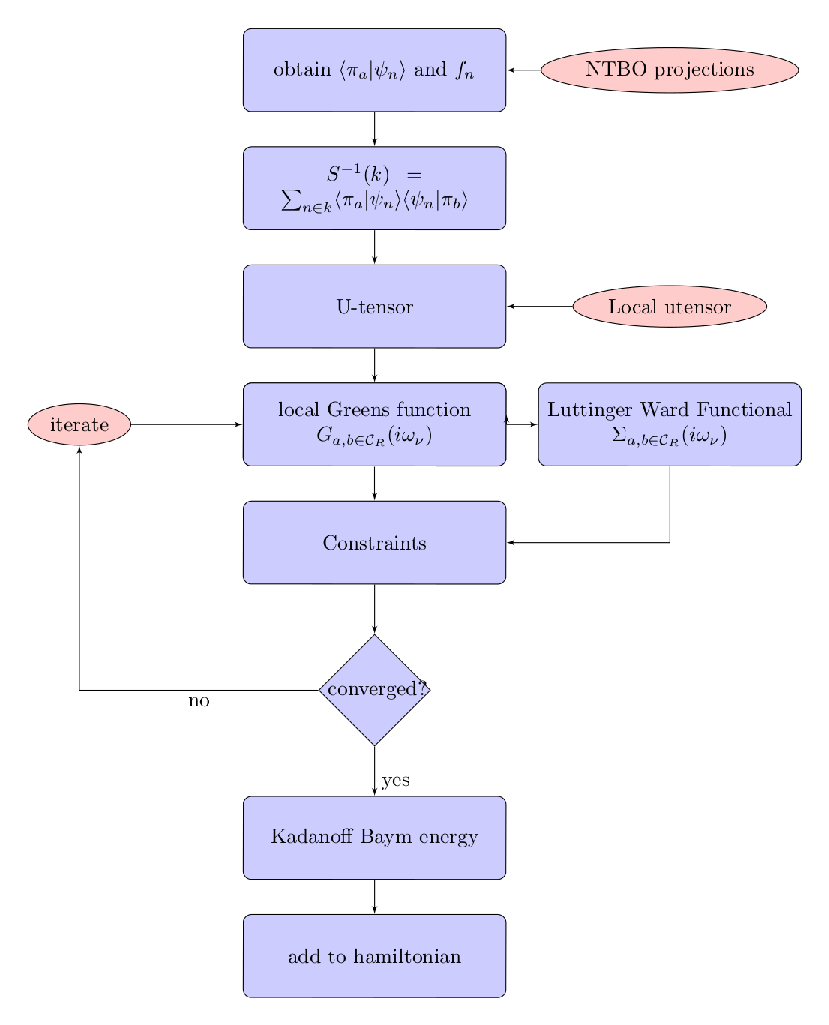
\includegraphics[width=0.5\linewidth]
{Figs/TikZ/FlowdiagramDMFTinterface/flow.eps}
\end{center}

%====================================================================
\subsection{Data exchange of the Object wit the outer world}
%====================================================================


%====================================================================
\subsection{DMFT\$GREEN}
%====================================================================
DMFT\$GREEN is the main subroutine of the DMFT object. It is called
from the LMTO object, which also provides the  projections onto the
tight-binding orbitals.

\begin{verbatim}
call dmft_ini()
call dmft_collecthamiltonian()  
call dmft_collectfulldenmat()  
call dmft_utensor() 
call dmft_smat()
call dmft_natorb()
call dmft_hrho()
call dmft_constraints('hrho')
do iter=1,3
  call dmft_gloc_withatomset() 
  call dmft_solver(etot) 
  call dmft_constraints('h0')
enddo ! end of loop over iterations to enforce constraint
call dmft_detot(svar)
etot=etot+svar      
call energylist$set('dmft interface',etot)
call energylist$add('local correlation',etot)
call energylist$add('total energy',etot)
call dmft_addtohpsi()
\end{verbatim}

\begin{enumerate}
\item \verb|DMFT_COLLECTHAMILTONIAN|:
\begin{eqnarray}
\langle\pi_a|\psi_n\rangle&&
\\
\rho_{a,b}(\vec{k})=\sum_n
\langle\pi_a|\psi_n(\vec{k})\rangle f_n(\vec{k})
\langle\psi_n(\vec{k})|\pi_b\rangle
\end{eqnarray}
%
\item \verb|DMFT_COLLECTFULLDENMAT|: Calculates the local density matrix,
  but for all orbitals on each atom. This is needed for the double
  counting term.
%
\item \verb|DMFT_UTENSOR|: 
\begin{eqnarray}
U_{a,b,c,d}=\alpha\int d^4x\int d^4x'\;
\frac{e^2\chi^*_a(\vec{x})\chi^*_b(\vec{x'})\chi_c(\vec{x})\chi_d(\vec{x'})}
{4\pi\epsilon_0|\vec{r}-\vec{r'}|}
\label{eq:defutensordmftobject}
\end{eqnarray}
Only the U-tensor for equal spin-electrons is stored. $\alpha$ is a
scale factor that mimics the screening of the U-tensor. It is called
\verb|LHFWEIGHT|.
%
\item \verb|DMFT_SMAT|:
\begin{eqnarray}
\mat{S}^{-1}(\vec{k})
=\sum_n\langle\pi_a|\psi_n(\vec{k})\rangle\langle\psi_n(\vec{k})|\pi_b\rangle
\end{eqnarray}
Note that the inverse overlap matrix is spin and orbital dependent.
$\mat{S}(\vec{k})$ and $\mat{S}^{-1}(\vec{k})$ are put on the KSET
structure.
%
\item \verb|DMFT_NATORB|: Construct a set of local, orthonormal orbitals
  $|\phi\rangle$. 


Ther atomicn natural orbitals are the eigenstates o9f, which are defined by
\begin{eqnarray}
\sum_{a,b}
\langle\phi_i|\pi_a\rangle\Bigl(\mat{S}_R\Bigr)_{a,b}
\langle\pi_b|\phi_j\rangle=\delta_{i,j}
\end{eqnarray}
where $\mat{S}_R$ is the local overlap operator obtained from
projection of $\sum_{\vec{k}} w_{\vec{k}}\mat{S}^{-1}(\vec{k})$ onto the
local orbitals and inversion of the projection matrix.


Construct transformation matrices
  $\langle\chi|\phi\rangle$ and $\langle\pi|\phi\rangle$ onto an
  orthonormal local basisset $|\phi\rangle$, so that 
\begin{eqnarray}
\sum_{a,b}
\langle\phi_i|\pi_a\rangle\Bigl(\mat{S}_R\Bigr)_{a,b}
\langle\pi_b|\phi_j\rangle=\delta_{i,j}
\end{eqnarray}
where $\mat{S}_R$ is the local overlap operator obtained from
projection of $\sum_{\vec{k}} w_{\vec{k}}\mat{S}^{-1}(\vec{k})$ onto the
local orbitals and inversion of the projection matrix.

The two matrices are related by
\begin{eqnarray}
\langle\pi|\phi\rangle=\mat{S}^{-1}_R\langle\pi|\phi\rangle
\end{eqnarray}

Alternatively, (using a hard-wired switch) on can select a
transformation onto natural orbitals, that is a representation for
which also the local density matrix is diagonal.
\begin{eqnarray}
\mat{\rho}_R\langle\chi|\phi\rangle=\mat{S}^{-1}_R
\langle\chi|\phi\rangle \vec{x}
\end{eqnarray}

The transformation matrices are stored in the fully non-collinear data
model in \verb|atomset%natorb%piphi| and \verb|atomset%natorb%chiphi|.
%
\item \verb|DMFT_HRHO|: For each k-point solve the generalized
  eigenvalue problem
\begin{eqnarray*}
\mat{\rho}(k)\mat{V}(\vec{k})=
\mat{S}^{-1}(\vec{k})\mat{V}(\vec{k})\mat{f}(\vec{k})
\end{eqnarray*}
where the $\mat{f}_k$ is a matrix that contains k-dependent
occupations, which differs from the occupations $f_n$.
\begin{eqnarray}
\mat{h}_\rho(\vec{k})-\mu=\mat{V}^{\dagger,-1}(\vec{k})\; k_B
\ln\left[
\frac{\mat{1}-\mat{V}^\dagger(\vec{k})\mat{\rho}(\vec{k})\mat{V}(\vec{k})}
{\mat{V}^\dagger(\vec{k})\mat{\rho}(\vec{k})\mat{V}(\vec{k})}
\right]\mat{V}^{-1}(\vec{k})
\end{eqnarray}
$\mat{h}_\rho$ is kept as \verb|KSET%HRHO|.
%
\item \verb|DMFT_CONSTRAINTS|: Determines $\mat{h}'(\vec{k})$ such that
\begin{eqnarray}
\mat{\rho}(\vec{k})=k_BT\sum_\nu \Bigl[(i\omega_\nu+\mu)\mat{S}(\vec{k})-
\mat{h'}-\mat{\Sigma}(i\omega_\nu)\Bigr]^{-1}
\end{eqnarray}
$\mat{h'}$ is kept as \verb|KSET%H0|.
%
\item \verb|DMFT_GLOC|: The local Green's function is obtained as
  Brillouin zone integral over the k-dependent greens function after
  projecting onto the correlated orbitals on the specified site.
\begin{eqnarray}
\mat{G}_R(i\omega_\nu)=\sum_k w(\vec{k})
\Bigl[(i\omega_\nu+\mu)\mat{S}(\vec{k})-
\mat{h'}-\mat{\Sigma}(i\omega_\nu)\Bigr]^{-1}_R
\end{eqnarray}

The result and its Laurent expansion terms are stored in
\verb|atomset%gloc| and \verb|atomset%gloclaur|.
%
\item \verb|DMFT_SOLVER|: Calculates the self energy for the local
  Green's functions. The Hartree-Fock term is separated out and
  calculated directly. Only the dynamic contribution is taken from an
  external solver. The double counting term is calculated as in the
  LMTO module. \textbf{For the double counting in the HF approximation
    only the exchange part is removed, while here also the correlation
    contribution should be taken out, because that is explicitly
    added.}

  The Hartree-Fock contribution is added directly to the double
  counting term. Thus the self energy \verb|atomset%sigma| is only
  the dynamical contribution.

Green's function and U-tensor are transformed into the representation
of orthonormal local orbitals, and the self-energy is transformed back
accordingly.

The external solver shall evaluate
\begin{eqnarray}
\Phi^{LW}[\mat{G}(i\omega_\nu),\hat{W}]
-\Phi^{LW,HF}[\mat{G}(i\omega_\nu),\hat{W}]
\end{eqnarray}
where
\begin{eqnarray}
  \Phi^{LW,HF}[\mat{G},\hat{W}]
  &=&
  \frac{1}{2}
  \frac{1}{\beta^{2}} 
  \sum_{\nu,\nu'} e^{i \beta \hbar \omega_\nu 0^{+}} e^{i \beta \hbar \omega_{\nu'} 0^{+}}
  \sum_{a,b,c,d}
  U_{a,b,d,c} 
  \nonumber\\ 
  &&\hspace{-1.2cm}\times\Big(
  G_{d,a}(i\omega_\nu)G_{c,b}(i\omega_{\nu'})
  -  G_{c,a}(i\omega_\nu)G_{d,b}(i\omega_{\nu'})
  \Big) 
\nonumber\\
&=& \frac{1}{2}
  \sum_{a,b,c,d}
  U_{a,b,d,c} \Bigl(
  \rho_{d,a}\rho_{c,b} -  \rho_{c,a}\rho_{d,b}\Bigr)
  \Big) 
\end{eqnarray}
Correspondingly, the self energy to be returned must have the
Hartree-Fock term subtracted out. That is, the double counting term
must be the Hartree-Fock term.
\begin{eqnarray*}
\Sigma_{a,b}(i\omega_\nu)=\frac{\beta\partial\Phi^{LW}}
{\partial G_{b,a}(i\omega_\nu)}-\sum_{c,d}\Bigl(U_{a,c,b,d}-U_{a,c,d,b}\Bigr)
\rho_{d,c}
\end{eqnarray*}

The external solver may make approximations to the U-tensor or to the
Kadanoff-Baym functional. However, they need to be consistent for
Luttinger-Ward functional and the corresponding Hartree-Fock
term. Thus, it is ensured that there is no approximation made beyond
the dynamic effects.

%
\item \verb|DMFT_DETOT|: Adds the non-local contribution to the total energy
\begin{eqnarray}
&-&\frac{1}{\beta}\sum_\nu\Tr\Bigl\lbrace
\ln\Bigl[
\mat{1}-
\Bigl(i\hbar\omega_\nu+\mu)\mat{1}-\mat{h}_{\rho}\Bigr)^{-1}
\Bigl(\mat{h}'+\mat{\Sigma}(i\omega_\nu)-\mat{h}_{\rho}\Bigr)
\Bigr]
\nonumber\\&&
+(\mat{h}'+\mat{\Sigma}(i\omega_\nu)-\mat{h}_\rho)\mat{G}(i\omega_\nu)
-
\Bigl[
\mat{G}(i\omega_\nu)
-\Bigl(i\hbar\omega_\nu+\mu)\mat{1}-\mat{h}_{\rho}\Bigr)^{-1}
\Bigr]
\Bigl(\mat{h}'-\mat{h}_\rho\Bigr)\Bigr\rbrace
\end{eqnarray}
\begin{itemize}
  \item \textbf{At this point I am still using the Dahlen trick.}  
  \item \textbf{Is it correct that only the dynamic self energy is used?}
\end{itemize}
%
\item \verb|DMFT_ADDTOHPSI|: Adds the energy derivative to
  \verb|this%htbc| of the \verb|waves_module|. There are two
  contributions, a k-dependent term which is restricted to the
  correlated orbitals and an site-dependent term that acts on all
  local orbitals.
\begin{itemize}
\item The site-specific term contains the double counting term for the
  DFT functional and the Hartree-Fock contribution to the self energy.
\end{itemize}
\end{enumerate}



%====================================================================
\subsection{DMFT\_INI}
%====================================================================

%====================================================================
\subsubsection{Hardwired data}
%====================================================================
\begin{itemize}
\item NOMEGA ($N_\omega$)
\end{itemize}

%====================================================================
\subsubsection{Inherited data}
%====================================================================
\begin{itemize}
\item NDIM from \verb|waves_module|
\item NSPIN from \verb|waves_module|
\item NKPTL from \verb|waves_module|
\item NAT  from \verb|ATOMLIST| Object
\item isp(IAT)
\item WKPT and (NKPT,KMAP) from \verb|DYNOCC| Object
\item KBT from \verb|dynocc$getr8a('temp')| from
  \verb|paw_occupations.f90|
\item \verb|atomset(iat)%lhfweight| from \verb|lmto_module|
\end{itemize}

%====================================================================
\subsubsection{Derived data}
%====================================================================
\begin{itemize}
\item NDIMD (=1 for NDIM=1,NSPIN=1; =2 for NDIM=1,NSPIN=2; =4 for
  NDIM=2,NSPIN=1)
\item List of positive Matsubara frequencies
\begin{eqnarray}
\omega_\nu=(2\nu-1)\pi k_BT \qquad\text{for $\nu=1,\ldots,N_\omega$}
\end{eqnarray}
\item Atomset structure
\begin{center}
 \begin{tabular}{ll}
 \verb|atomset\%nloc| & number of correlated orbits on this atom \\
\verb|atomset\%ICHI1| & first value of ICHI index for this atom\\
\verb|atomset\%ICHI2| & last value of ICHI index for this atom\\
\end{tabular}
\end{center}
%
\item KSET structure
\begin{center}
 \begin{tabular}{ll}
 \verb|KSET\%WKPT| & geometric k-point weight\\
\end{tabular}
\end{center}
\end{itemize}

%====================================================================
\subsection{DMFT\_UTENSOR}
%====================================================================
Obtain the onsite Utensor for all local orbitals from subroutine
\verb|dmft_ulocal| reduces it to the entries for the correlated
orbitals.

In \verb|DMFT_ULOCAL| it obtains the local U-tensor from the
\verb|POTPAR%TAILED%U| and \verb|SBAR| of the LMTO Object. This object
contains the extended $\phi$ and $\dot{\phi}$ functions
\begin{eqnarray}
|\chi_a\rangle=|\phi_a\rangle-
\sum_{b; R_b=R_a}|\dot{\bar{\phi}}_b\rangle \bar{S}_{a,b}
\end{eqnarray}


The U-tensor is constructed in \verb|LMTO\_MAKETAILEDPARTIALWAVES|.
\verb|LMTO\_ULITTLE| constructs
\begin{eqnarray}
u_{\ell,a,b,c,d}
=\frac{2\ell+1}{4\pi}
\int dr\; r^2R_c(r)R_d(r)\Bigl[\int d^3r'\;V_\ell(r,r')R_a(r')R_b(r')\Bigr]
\end{eqnarray}
where the kernel $V_\ell(r,r')$ is the one used by $RADIAL\$POISSON$.
\textbf{There is a input parameter that determines which $\ell$ values are
considered.}

In \verb|LMTO_UTENSOR| the U-tensor elements are composed according to
\begin{eqnarray}
U_{a,b,c,d}=\sum_{ell}\frac{4\pi}{2\ell+1}\sum_{m=-\ell}^\ell
u_{\ell,b,d,c,a} C_{L,L_b,L_d}C_{L,L_c,L_a}
\end{eqnarray}

The U-tensor is screened by a factor \verb|LHFWEIGHT|. It is obtained
from the \verb|lmto_module| either as the global value \verb|HFWEIGHT|
or the individual value from hybridsetting. This very same factor is
used for the double counting term.

Thus the U-tensor is defined as\footnote{$\vec{x}=(\vec{r},\sigma)$}
in Eq.~\ref{eq:defutensordmftobject}, i.e. as
\begin{eqnarray}
U_{a,b,c,d}=\int d^4x\int d^4x'\;
\frac{e^2\chi^*_a(\vec{x})\chi^*_b(\vec{x'})\chi_c(\vec{x})\chi_d(\vec{x'})}
{4\pi\epsilon_0|\vec{r}-\vec{r'}|}
\end{eqnarray}
The U-tensor contributes only if $\sigma_a=\sigma_c$ and if
$\sigma_b=\sigma_d$.
With this definition the Hartree and exchange  energy have the form
\begin{eqnarray}
E_H=\frac{1}{2}\sum_{a,b,c,d}U_{a,b,c,d}\;\rho_{c,a}\rho_{d,b}
\nonumber\\
E_X=\frac{1}{2}\sum_{a,b,c,d}U_{a,b,c,d}\;\rho_{c,b}\rho_{d,a}
\end{eqnarray}


%====================================================================
\subsection{DMFT\_NATORB}
%====================================================================
Construct natural orbitals in the space of correlated orbitals on one
site.

For this purpose, I redefine the unity operator for the sub Hilbert
space of correlated orbitals.
\begin{eqnarray}
\hat{1}_{\mathcal{C}_R}
=\sum_{\alpha,\beta}\sum_n
|\chi_\alpha\rangle
\langle\pi_\alpha|\psi_n\rangle\langle\psi_n|\pi_\beta\rangle
\langle\chi_\beta|
\end{eqnarray}
which allows one to identify the inverse overlap matrix in this sub-Hilbert space.
\begin{eqnarray}
\mat{S}^{-1}_{\alpha,\beta}
=\sum_{\alpha,\beta}\sum_n
\langle\pi_\alpha|\psi_n\rangle\langle\psi_n|\pi_\beta\rangle
\end{eqnarray}
Note,however, that this matrix lives only on a single site! We can
obtain it from the k-dependent $\mat{S}^{-1}$ by summing over k-points
and cutting out the corresponding submatrix. However, it is not
allowed to do the same thing for the overlap matrix itself!

The one-particle density matrix in this sub-Hilbert space has the form
\begin{eqnarray}
\hat{\rho}_{\mathcal{C}_R}
=\sum_{\alpha,\beta}\sum_n
|\chi_\alpha\rangle
\langle\pi_\alpha|\psi_n\rangle f_n \langle\psi_n|\pi_\beta\rangle
\langle\chi_\beta|
\end{eqnarray}

The eigenvalue equation
\begin{eqnarray}
\hat{\rho}|\phi_n\rangle=|\phi_n\rangle f_n
\nonumber\\
\sum_{\alpha,\beta}|\chi_\alpha\rangle
\langle\pi_\alpha|\hat{\rho}|\pi_\beta\rangle\langle\chi_\beta|\phi_j\rangle
=\sum_{\alpha,\beta}|\chi_\alpha\rangle\langle\pi_\alpha|\pi_\beta\rangle
\langle\chi_\beta|\phi_j\rangle f_j
=\sum_{\alpha,\beta}|\chi_\alpha\rangle
\mat{S}^{-1}_{\alpha,\beta}\langle\chi_\beta|\phi_j\rangle \bar{f}_j
\end{eqnarray}
provides us with a new set of occupations $\bar{f}$ of local natural
orbitals and eigenvectors
$\langle\chi_\beta|\phi_j\rangle=V_{\beta,j}$.
\begin{eqnarray}
\mat{\rho}\mat{V}=\mat{S}^{-1}\mat{V}\bar{f}
\qquad\text{with}\qquad
\mat{V}^\dagger\mat{S}^{-1}\mat{V}=\mat{1}
\end{eqnarray}

The natural orbitals are
\begin{eqnarray}
|\phi_j\rangle=\sum_{\alpha,\beta\in\mathcal{C}_R}
\underbrace{|\chi_\alpha\rangle
\mat{S}^{-1}_{\alpha,\beta}\langle\chi_\beta|}_{\mat{1}_{\mathcal{C}_R}}
\phi_j\rangle
=\sum_{\alpha\in\mathcal{C}_R}|\chi_\alpha\rangle
\underbrace{\Bigl(\mat{S}^{-1}\mat{V}\Bigr)_{\alpha,j}}_{\mat{V}^{\dagger,-1}_{\alpha,j}}
\end{eqnarray}

The matrix $\mat{V}$ is placed into the structure
\verb|atomset%natorb%chiphi|, together with the occupations $\bar{f}$
which are in \verb|atomset%natorb%f|. In addition we store
$\mat{S}^{-1}\mat{V}=\mat{V}^{\dagger,-1}$ in
\verb|atomset%natorb%piphi| All data in \verb|atomset%natorb| are
stored in the fully non-collinear model.

%====================================================================
\subsection{DMFT\_HRHO}
%====================================================================
The conversion of occupations into energies is done in the routine
\verb|DMFT_EOFF|.
\begin{eqnarray}
\epsilon=k_B
\begin{cases}
\ln\left(\frac{1-f}{f}\right) &\text{for $f_0<f<1-f_0$}\\
a+b(f-f_0)&\text{for $f<f_0$}\\
-a+b(f-(1-f_0))&\text{for $f>1-f_0$}\\
\end{cases}
\end{eqnarray}
where $a$ and $b$ are determined such that the mapping is
differentiable. The value of $f_0$ is currently set to $10^{-6}$.

%====================================================================
\subsection{DMFT\_CONSTRAINTS}
%====================================================================
The two equations are solved iteratively
\begin{eqnarray}
\bar{\mat{\rho}}(\vec{k})&=&k_BT\sum_\nu
\underbrace{\Bigl[
(i\omega_\nu+\mu)\mat{S}(\vec{k})-\mat{h}(\vec{k})-\sum_R \Sigma_R(i\omega_\nu)
\Bigr]^{-1}}_{\mat{G}(\vec{k})}
\\
\delta\mat{h}&=&4k_BT\mat{S}(\vec{k})\Bigl[
\bar{\rho}(\vec{k})-\rho(\vec{k})\Bigr]
\mat{S}(\vec{k})
\end{eqnarray}

This equation is a Newton scheme with the Green's function in the
slope estimate replaced by the non-interacting Green's function with
zero potential self energy and chemical potential. \textbf{Should
  there be convergence problems, it may be improved by using the
  static Green's function $\mat{G}_\rho$ instead.}



The Laurent expansion terms are
\begin{eqnarray}
\mat{G}^{(1)}(\vec{k})&=&\mat{S}^{-1}(\vec{k})
\nonumber\\
\mat{G}^{(2)}(\vec{k})&=&\mat{S}^{-1}(\vec{k})
\Bigl(-\mu\mat{S}(\vec{k})+\mat{h'}(\vec{k})+\mat{\Sigma}^{(1)}(\vec{k})
\Bigr)
\mat{S}^{-1}(\vec{k})
\nonumber\\
\mat{G}^{(2)}(\vec{k})&=&
\mat{S}^{-1}(\vec{k})
\biggl[
\mat{S}^{-1}(\vec{k})
\Bigl(-\mu\mat{S}(\vec{k})+\mat{h'}(\vec{k})+\mat{\Sigma}^{(1)}(\vec{k})
\Bigr)
\mat{S}^{-1}(\vec{k})+\mat{\Sigma}^{(2)}(\vec{k})
\biggr]
\mat{S}^{-1}(\vec{k})
\nonumber\\
\end{eqnarray}


%====================================================================
\subsection{DMFT\_SOLVER}
%====================================================================
The solver first calculates the Hartree-Fock contribution to the
Luttinger-Ward functional as defined in Eq.~\ref{eq:philwhf} and the
corresponding self energy. Because the Hartree-Fock self energy is
static and because it does not affect the density matrix constraint,
it is added together with the double counting correction to
\verb|atomset%denmat%h|.


Then the double counting correction is calculated. \textbf{At the
  moment we still subtract out only the exchange part, which is
  consistent with the hybrid functionals but not as double counting
  for correlation.}

Finally the data are prepared for the solver in
\verb|DMFT_dynamicsolver|. The dynamicsolver transforms all data into
a spin-orbital representation of orthonormal states, which may be
either natural orbitals derived from the local density matrix or which
may be eigenstates of the local overlap matrix.

%====================================================================
%\section{Helper routines}
%====================================================================

\appendix
%====================================================================
%\chapter{Helper routines}
%====================================================================
%====================================================================
\chapter{Matsubara frequencies}
\label{app:matsubarafreq}
%====================================================================

The Matsubara frequencies for Fermions are
\begin{eqnarray*}
\omega_\nu=(2\nu+1)\frac{\pi}{\hbar\beta}
\end{eqnarray*}

A Matsubara sum has the general form
\begin{eqnarray*}
\frac{1}{\beta}\sum_{\nu\in z} g(i\omega_\nu)
\end{eqnarray*}
where $g(i\omega_\nu)$ is a analytic function.

%====================================================================
\section{Evaluation using residual theorem}
%====================================================================
In order to evaluate the Matsubara sum we introduce a
\textbf{Matsubara weighting functions}\index{ Matsubara weighting
  functions}, that has simple poles at $i\omega_\nu$, so that we can
exploit the residuum theorem. For Fermions, two such weighting
functions are used
\begin{eqnarray}
h^\pm(z)=\frac{\mp\beta\hbar}{1+\e{\pm\beta\hbar z}}
\end{eqnarray}

The poles of the Matsubara weighting functions obey
\begin{eqnarray}
1+\e{\pm\beta\hbar z}=0
\label{eq:matsubarapolecond}
\end{eqnarray}
With the help of
\begin{eqnarray*}
\e{\pm\beta\hbar z}
=\e{\pm\beta\hbar\Re(z)}\e{\pm i\beta\hbar\Im(z)}
=\e{\beta\hbar\Re(z)}\cos(\beta\hbar\Im(z))
\pm i\e{\beta\hbar\Re(z)}\sin(\beta\hbar\Im(z))
\end{eqnarray*}
\eq{eq:matsubarapolecond} can be rewrfitten in the form
\begin{eqnarray}
\Rightarrow
\e{\pm \beta\hbar\Re(z)}\cos(\beta\hbar\Im(z))=-1
\qquad\text{and}\qquad
\e{\pm \beta\hbar\Re(z)}\sin(\beta\hbar\Im(z))=0
\end{eqnarray}
The second equation is obeyed for
\begin{eqnarray}
\Im(z)=\frac{n\pi}{\hbar\beta}\qquad\text{for arbitrary integer $n$}
\end{eqnarray}
The first equation yields
\begin{eqnarray}
-1&=&\e{\pm\beta\hbar\Re(z)}\cos(\beta\hbar\Im(z))
=\e{\pm\beta\hbar\Re(z)}\cos(n\pi)
=\e{\pm\beta\hbar\Re(z)}(-1)^n
\nonumber\\
\Rightarrow
n-1&=&2\nu \qquad\text{for arbitrary integer $\nu$, and $Re(z)=0$}
\nonumber\\
\Rightarrow
n&=&2\nu+1
\end{eqnarray}
Thus we obtain that the poles of the Matsubara weighting function lie
at the Matsubara frequencies.
\begin{eqnarray}
z_\nu=i(2\nu+1)\frac{\pi}{\hbar\beta}=i\omega_\nu
\end{eqnarray}

Next we need to show that the weighting function at the poles behaves
like $\frac{1}{z-z_0}+O(|z-z_0|^2)$, where $x_0$ is the position of the pole.
For this purpose we expand the inverse
\begin{eqnarray}
\frac{1}{\mp\hbar\beta}(1+\e{\pm\hbar\beta z})
&=&\frac{1}{\mp\hbar\beta}
(\underbrace{1+\e{\pm\hbar\beta z_0}}_{=0} 
\pm\hbar\beta\underbrace{\e{\pm\hbar\beta z_0}}_{-1}(z-z_0)+O(|z-z_0|^2) )
\\
&=&(z-z_0)+O(|z-z_0|^2) 
\end{eqnarray}



With the help of the Matsubara weighting function we can evaluate the
Matsubara sum as\footnote{Cauchy's Integral formula:
\begin{eqnarray*}
Res(f,z_0)=\frac{1}{2\pi i}\oint_\gamma dz\; f(z)
\end{eqnarray*}
where $\gamma$ is a counter-clockwise countour around a pole $z_0$ of
a function $f$, that can be expanded into a Laurent series about
$z_0$. The Residuum is the prefactor of the term $1/(z-z_0)$ in the
Laurent expansion.}
\begin{eqnarray}
\frac{1}{\beta}\sum_{nu\in Z}g(i\omega_\nu)&=&
\frac{1}{2\pi i\beta}\oint g(z) h^{\pm}(z)
=-\frac{1}{\beta}\sum_{z_0\in\text{poles of g}}
\text{Res}(gh^{\pm},z_0)
\end{eqnarray}





The minus sign occurs because the c ounter clockwise integration of
the contur in the half plane turns into a clock-wise integration about
the pole.

\begin{center}
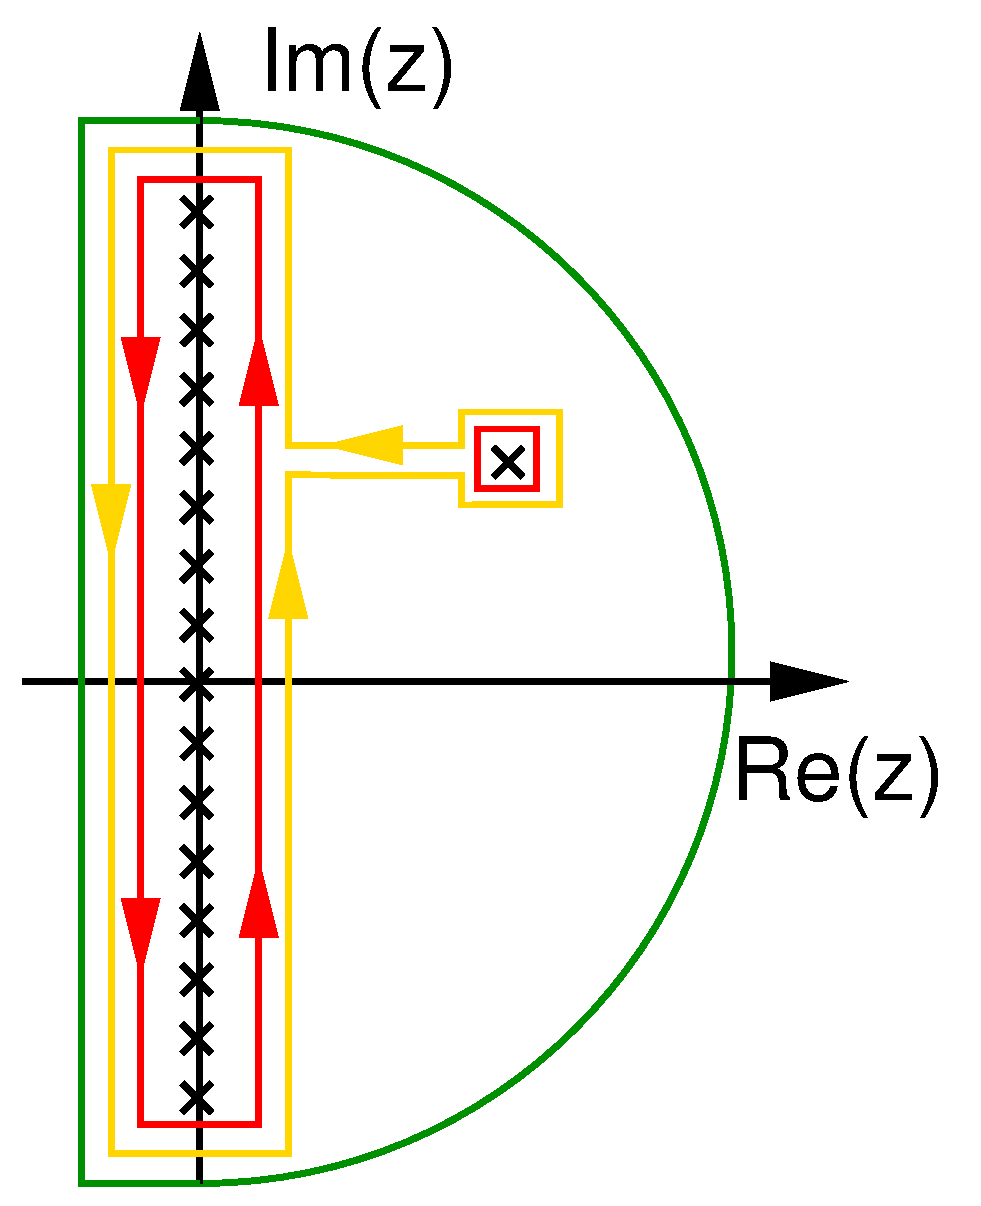
\includegraphics[width=0.25\linewidth]{Figs/Xfig/Matsubaracontour/contour.eps}
\end{center}

The integration is closed in the half plane with $\pm Re(z)>0$, because
we there the corresponding weighting function $h^{\pm}$ decays
exponentially for $Re(z)\rightarrow\pm\infty$.


%====================================================================
\subsection{Matsubara sums}
%====================================================================
From \url{http://en.wikipedia.org/wiki/Matsubara_frequency} we obtain
the following expression for the \textbf{fermionic} summations.  In
these expressions the Matsubara frequencies are\footnote{They differ
  from those of the source by a factor $1/\hbar$.}
\begin{eqnarray}
\omega_\nu=(2\nu+1)\pi/(\hbar\beta)
\end{eqnarray}


\begin{eqnarray}
-k_BT\sum_\nu\ln[-i\hbar\omega_\nu+\epsilon]\e{i\omega_\nu0^+}
&=&-k_BT\ln[1+e^{-\beta \epsilon}]
\\
k_BT\sum_\nu \frac{1}{(i\hbar\omega_\nu-\epsilon)}\e{i\omega_\nu 0^+}
&=&(1+\e{\beta \epsilon})^{-1}
\\
k_BT\sum_\nu \frac{1}{(i\hbar\omega_\nu-\epsilon)^n}
&=&\frac{1}{(k_BT)^{n-1}(n-1)!}
\left.\partial_\epsilon^{n-1}\right|_{x=\beta\epsilon}(1+\e{x})^{-1}
\end{eqnarray}
\begin{center}
\begin{tabular}{|c|c|c|c|c|c|c|c|c|c|c|}
\hline
$j$& 1 & 2 & 3 & 4 & 5 &6 &7 &8 & 9 & 10\\
\hline
$\partial^{j-1}_x(1+\e{x})^{-1}$
&$\frac{1}{2}$ 
&$-\frac{1}{4}$ 
&$0$ 
&$+\frac{1}{8}$ 
&$0$ 
&$-\frac{1}{4}$ 
&$0$ 
&$\frac{17}{16}$
&$0$ 
&$-\frac{31}{4}$
\\
\hline
$\partial^{j-1}_x(1+\e{x})^{-1}$
&$0.5$ 
&$-0.25$ 
&$0$ 
&$+0.125$ 
&$0$ 
&$-0.25$ 
&$0$ 
&$+1.0625$
&$0$ 
&$-7.75$
\\
\hline
\hline
$j$& 11 & 12 & 13 & 14 & 15 &16 &17 &18 & 19 & 20\\
\hline
$\partial^{j-1}_x(1+\e{x})^{-1}$
&$0$ 
&$\frac{691}{8}$ 
&$0$ 
&$-\frac{5461}{4}$ 
&$0$ 
&$\frac{929569}{32}$ 
&$0$ 
&$-\frac{3202291}{4}$
&$0$ 
&$+\frac{221930581}{8}$
\\
\hline
$\partial^{j-1}_x(1+\e{x})^{-1}$
&$0$ 
&$86.375$ 
&$0$ 
&$-1365.25$ 
&$0$ 
&$29.0\times10^3$ 
&$0$ 
&$-800\times10^3$
&$0$ 
&$27.7\times 10^6$ %$+27741322.625$
\\
\hline
\end{tabular}
\end{center}

\begin{figure}[h!]
\begin{center}
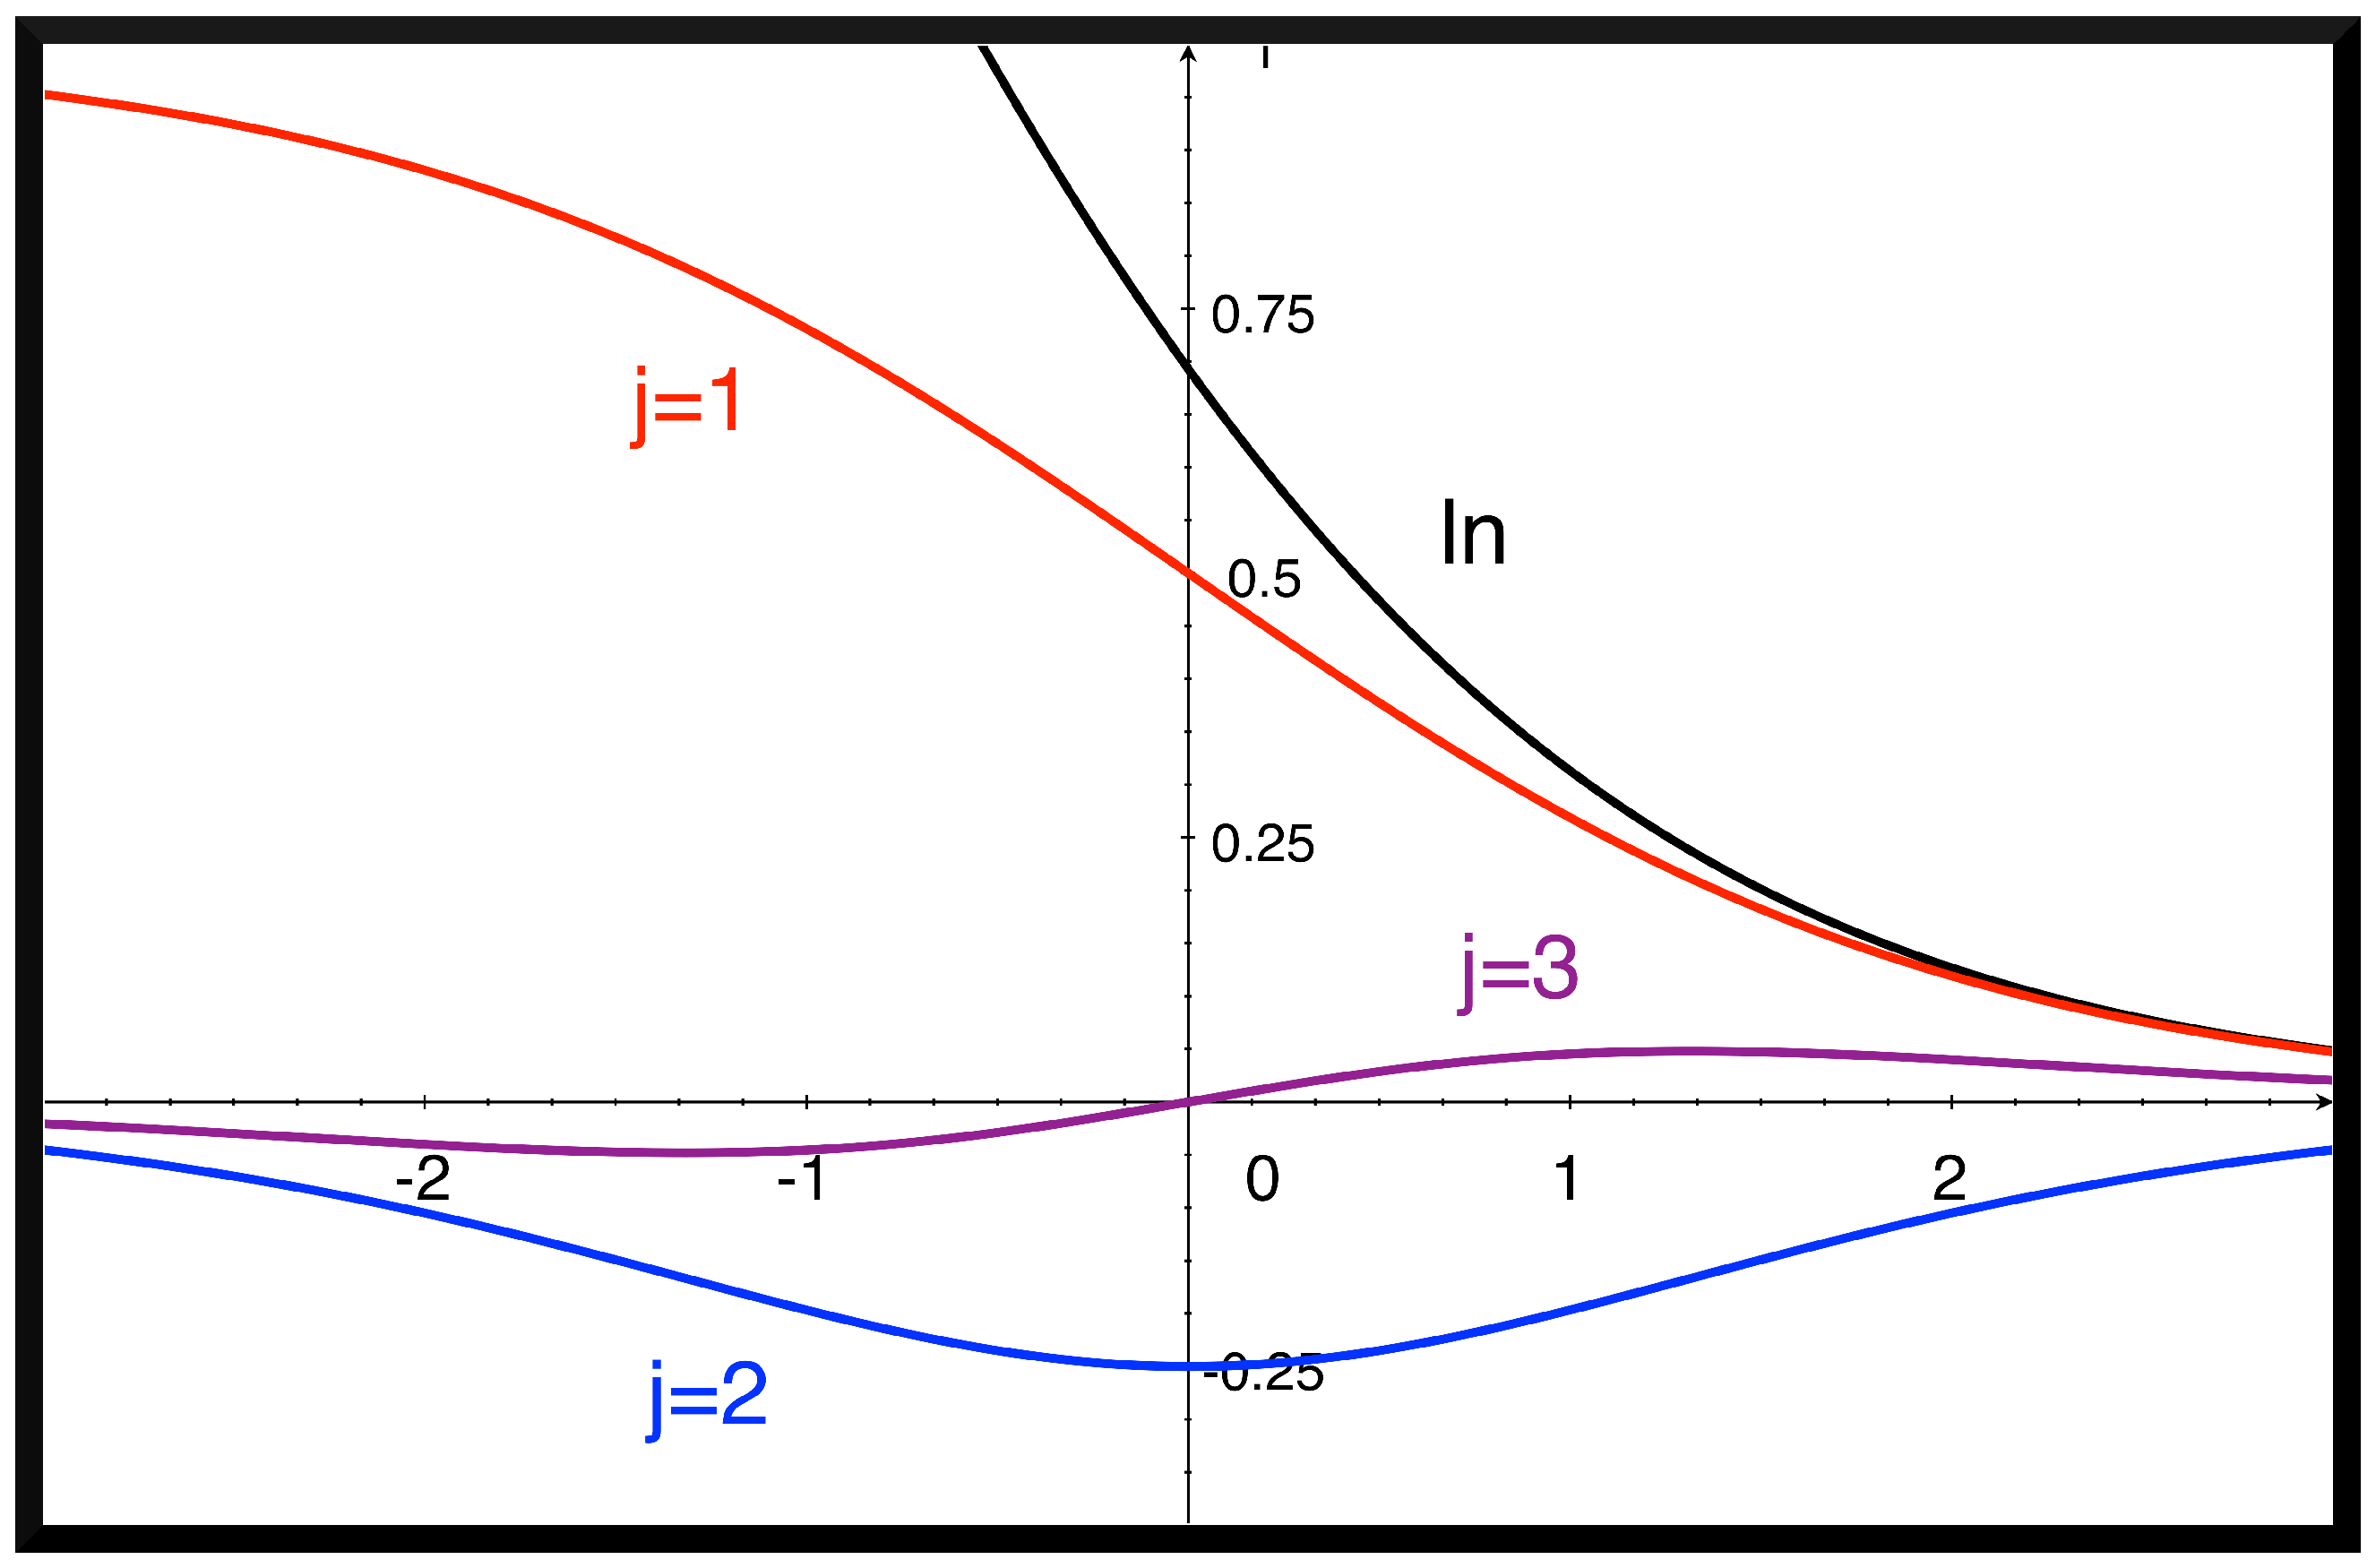
\includegraphics[width=0.8\linewidth,clip=true]
{Figs/Matsubarasums/matsubarasums1.eps}
\end{center}
\caption{\label{fig:matsubarasums} The result of Matsubara sums
  $-k_BT\sum_\nu\ln[-i\hbar\omega_\nu+\epsilon]$, $k_BT\sum_\nu
  \frac{1}{(i\hbar\omega_\nu-\epsilon)}\e{i\omega_\nu 0^+}$,
$k_BT\sum_\nu \frac{1}{(i\hbar\omega_\nu-\epsilon)^2}$ as
  function of energy $\epsilon$.}
\end{figure}



%====================================================================
\subsection{Matsubara sums on finite grids}
%====================================================================
The finite Matsubara sums result in a Fermi function that does not
reach zero or one. In particular, in the limit of e level, that lies
far from the chemical potential, the finite Matsubara sum falls off to
$\frac{1}{2}$.

\begin{figure}[h!]
\begin{center}
\includegraphics[width=0.4\linewidth,clip=true]
{Figs/Xmgrace/FiniteMatsubara/gsumlow.eps}
\includegraphics[width=0.4\linewidth,clip=true]
{Figs/Xmgrace/FiniteMatsubara/gsumhigh.eps}
\end{center}
\caption{\label{fig:finfitematsubara} Fermi function calculated from a
  finite Matsubara sum. The function is shifted by $-\frac{1}{2}$
  because no relgularization has been done. The sums have been
  performed with $2^n$ grid points with $n=0,\ldots,12$ for $k_BT=1.$}
\end{figure}



%====================================================================
\chapter{The Green function}
%====================================================================
We construct the \textbf{lattice Green's function} defined as
\begin{eqnarray}
\hat{G}^{lat}(i\omega_\nu)&=&
\biggl[(i\hbar\omega_\nu+\mu)\hat{1}
-\hat{h}-\Delta\hat{\Sigma}(i\omega_\nu)\biggr]^{-1}
\nonumber\\
&\approx&\sum_{n,n'}|\psi_n\rangle
\underbrace{
\biggl[\langle\psi_{n'}|(i\hbar\omega_\nu+\mu)\hat{1}-\hat{h}
-\Delta\hat{\Sigma}(i\omega_\nu)|\psi_n\rangle\biggr]_{n,n'}^{-1}
}_{G^{lat}_{n,n'}}
\langle\psi_{n'}|
\label{eq:latgreenfunc}
\end{eqnarray}
This expression is approximate, if the set of band states is not
complete. In practice, corrections are required.

In the representation of the band states, the lattice Green's function
has the form
\begin{eqnarray}
G^{lat}_{n,n'}(i\omega_\nu)&=&
\biggl[\langle\psi_{n'}|(i\hbar\omega_\nu+\mu)\hat{1}-\hat{h}
-\Delta\hat{\Sigma}(i\omega_\nu)|\psi_n\rangle\biggr]_{n,n'}^{-1}
\label{eq:latgreenfuncmat}
\end{eqnarray}
Note, that the matrix to be inverted is not necessarily hermitean!

%====================================================================
\section{Generic properties}
%====================================================================
%====================================================================
\subsection{Green's function with negative Matsubara frequencies}
%====================================================================
Green's functions and self energies obey the relation
\begin{eqnarray*}
\mat{G}(-i\omega_\nu)=\mat{G}^\dagger(i\omega)
\end{eqnarray*}
This allows one to store only half of the Green's functions.

Proof:

\begin{eqnarray}
G_{\alpha,\beta}(i\omega_n)&=&
-\frac{1}{\hbar}\int_0^{\hbar\beta} d\tau\;\e{i\omega_n\tau}
\Bigl\langle\mathcal{T}\hat{c}_\alpha(\tau)\hat{c}^\dagger_\beta(0)\Bigr\rangle
\\
\Rightarrow
G_{\alpha,\beta}(-i\omega_n)
&=&
-\frac{1}{\hbar}\int_0^{\hbar\beta} d\tau\;\e{-i\omega_n\tau}
\Bigl\langle\mathcal{T}\hat{c}_\alpha(\tau)\hat{c}^\dagger_\beta(0)\Bigr\rangle
\nonumber\\
&=&
\biggl\lbrace
-\frac{1}{\hbar}\int_0^{\hbar\beta} d\tau\;\e{i\omega_n\tau}
\Bigl\langle\biggl(\e{\beta(\hat{H}-\mu\hat{N})}\hat{c}_\alpha
\e{-\beta(\hat{H}-\mu\hat{N})}\hat{c}^\dagger_\beta\biggr)^\dagger
\Bigr\rangle
\biggr\rbrace^*
\nonumber\\
&=&
\biggl\lbrace
-\frac{1}{\hbar}\int_0^{\hbar\beta} d\tau\;\e{i\omega_n\tau}
\Bigl\langle
\hat{c}_\beta\e{-\beta(\hat{H}-\mu\hat{N})}\hat{c}^\dagger_\alpha
\e{\beta(\hat{H}-\mu\hat{N})}
\Bigr\rangle
\biggr\rbrace^*
\nonumber\\
&\stackrel{cycl. perm}{=}&
\biggl\lbrace
-\frac{1}{\hbar}\int_0^{\hbar\beta} d\tau\;\e{i\omega_n\tau}
\Bigl\langle
\e{\beta(\hat{H}-\mu\hat{N})}
\hat{c}_\beta\e{-\beta(\hat{H}-\mu\hat{N})}\hat{c}^\dagger_\alpha
\Bigr\rangle
\biggr\rbrace^*
\nonumber\\
&=&
\biggl\lbrace
-\frac{1}{\hbar}\int_0^{\hbar\beta} d\tau\;\e{i\omega_n\tau}
\Bigl\langle
\mathcal{T}\hat{c}_\beta(\tau)\hat{c}^\dagger_\alpha
\Bigr\rangle
\biggr\rbrace^*
\nonumber\\
&=&
G_{\beta,\alpha}^*(i\omega_\nu)
\end{eqnarray}

%====================================================================
\subsection{Density of states}
%====================================================================
For a system of independent electrons, the number of particles is
related to the chemical potential via
\begin{eqnarray}
N(\mu)=\int_{-\infty}^\infty d\epsilon\; f_\mu(\epsilon) D(\epsilon)
\;,
\end{eqnarray}
where $D$ is the density of states. $f_\mu(\epsilon)$ is the Fermi function.

\begin{eqnarray}
\frac{dN}{d\mu}
&=&\int_{-\infty}^\infty d\epsilon\; 
\frac{\partial f_\mu(\epsilon)}{\partial\mu} D(\epsilon)
=
\underbrace{\int_{-\infty}^\infty d\epsilon\; 
\frac{\beta}{\cosh^2\Bigl(\frac{1}{2}\beta(\epsilon-\mu)\Bigr)} D(\epsilon)
}_{\tilde{D}(\mu)}
\end{eqnarray}
Thus $dN/d\mu$ provides us with a broadened density of states.

No we generalize the relation obtained for independent Fermions to
interacting Fermions. The number of states function $N_{a,b}(\mu)$ can
be obtained from the Green's function
\begin{eqnarray}
N_{a,b}(\mu)
&=&\frac{1}{\beta}\sum_\nu G_{a,b}(i\omega_\nu,\mu)\e{i\omega_\nu0^+}
=\frac{1}{\beta}\sum_\nu 
\biggl[
\Bigl(\mat{G}(i\omega_\nu,\mu_0)
\Bigr)^{-1}+(\mu-\mu_0)\biggr]^{-1}_{a,b}\e{i\omega_\nu0^+}
\end{eqnarray}

The smoothened density of states $\tilde{D}_{a,b}(\mu)$ is then
obtained as derivative with respect to $\mu$.
\begin{eqnarray}
\tilde{D}_{a,b}(\mu)&\defas&\frac{\partial N_{a,b}}{\partial\mu}
\nonumber\\
&=&
-\frac{1}{\beta}\sum_\nu 
\sum_c
\biggl[
\Bigl(\mat{G}(i\omega_\nu,\mu_0)
\Bigr)^{-1}+(\mu-\mu_0)\mat{1}\biggr]^{-1}_{a,c}
\biggl[
\Bigl(\mat{G}(i\omega_\nu,\mu_0)
\Bigr)^{-1}+(\mu-\mu_0)\mat{1}\biggr]^{-1}_{c,b}
\nonumber\\
\end{eqnarray}

%====================================================================
\section{Project Green's function onto local orbitals}
%====================================================================
For a Hamiltonian $\hat{h}=\sum_{a,b}|\pi_a\rangle
h_{a,b}\langle\pi_b|$ and a self energy 
$\hat{\Sigma}(i\omega_\nu)=
\sum_{a,b}|\pi_a\rangle
\Sigma_{a,b}(i\omega_\nu)
\langle\pi_b|$
acting on the local orbitals, the Green's function can be expressed
as
\begin{eqnarray}
\hat{G}(i\omega_\nu)&=&
\sum_{a,b}|\chi_a\rangle
\biggl\lbrace
\sum_n\langle\pi_a|\psi_n\rangle
\biggl[
(i\hbar\omega_\nu+\mu)\delta_{n,n'}
\nonumber\\
&&-\sum_{c,d}\langle\psi_n|\pi_c\rangle
\Bigl(h_{c,d}+\Sigma_{c,d}(i\omega_\nu)\Bigr)
\langle\pi_d|\psi_{n'}\rangle
\biggr]^{-1}_{n,n'}
\langle\psi_{n'}|\pi_b\rangle
\biggr\rbrace
\langle\chi_b|
\label{eq:greenlocorb}
\end{eqnarray}
We converted Eq.~\eqref{eq:latgreenfunc} into a basis of local
orbitals $|\chi_a\rangle$ using
$|\psi_n\rangle=\sum_a|\chi_a\rangle\langle\pi_a|\psi_n\rangle$.


In order to evaluate Green's function, we still need to refer to the
band states. The Green's function can, however, also be expressed
without making direct use of the band states, namely as
\begin{eqnarray}
\mat{G}_{a,b}(i\omega_\nu)
=\biggl[(i\hbar\omega_\nu+\mu)\mat{S}
-\mat{h}-\mat{\Sigma}(i\omega_\nu)\biggr]^{-1}
_{a,b}
\label{eq:greenlocform1}
\end{eqnarray}
where
\begin{eqnarray}
S^{-1}_{a,b}=\sum_k\langle\pi_a|\psi_n\rangle f_n\langle\psi_n|\pi_b\rangle
\label{eq:inverses}
\end{eqnarray}

\textbf{Proof:}
Here, I will show that the Green's function matrix 
\begin{eqnarray}
\mat{G}_{a,b}(i\omega_\nu)=
\sum_n\langle\pi_a|\psi_n\rangle
\biggl[
(i\hbar\omega_\nu+\mu)\delta_{n,n'}-
\sum_{c,d}\langle\psi_n|\pi_c\rangle
\Bigl(\mat{h}_{c,d}+\mat{\Sigma}_{c,d}(i\omega_\nu)\Bigr)
\langle\pi_d|\psi_{n'}\rangle
\biggr]^{-1}_{n,n'}
\langle\psi_{n'}|\pi_b\rangle
\nonumber\\
\label{eq:greenlocform2}
\end{eqnarray}
can be expressed in the form of \eq{eq:greenlocform1}.

I order to simplify the proof, I will not write out the self energy,
nor the chemical potential. This is possible because the proof works
for each Matsubara frequency independently, so that both can be
absorbed in the non-interacting Hamiltonian.
\begin{eqnarray}
G_{a,b}(i\omega_\nu)
&=&
\sum_{n,n'}\langle\pi_a|\psi_{n}\rangle
\biggl(i\hbar\omega_\nu\delta_{n,n'}
-
\langle\psi_n|\pi\rangle
\mat{h}
\langle\pi|\psi_{n'}\rangle\biggr)^{-1}_{n,n'}
\langle\psi_{n'}|\pi_b\rangle
\nonumber\\
&=&
\sum_{n,n'}\langle\pi_a|\psi_{n}\rangle
\biggl[
\sum_{j=0}^\infty
\frac{1}{(i\hbar\omega_\nu)^{j+1}}
\biggl(
\langle\psi|\pi\rangle
\mat{h}
\langle\pi|\psi\rangle\biggr)^j_{n,n'}
\biggr]\langle\psi_{n'}|\pi_b\rangle
\nonumber\\
&=&
\sum_{n,n'}\langle\pi_a|\psi_{n}\rangle
\biggl[
\sum_{j=0}^\infty
\frac{1}{(i\hbar\omega_\nu)^{j+1}}
\biggl(\sum_{n_2,\ldots,n_{j}} 
\langle\psi_{n}|\pi\rangle
\mat{h}
\langle\pi|\psi_{n_2}\rangle\langle\psi_{n_2}|\pi\rangle
\ldots
\mat{h}
\langle\pi|\psi_{n'}\rangle\biggr)\biggr]
\langle\psi_{n'}|\pi_b\rangle
\nonumber\\
&=&
\sum_{j=0}^\infty\frac{1}{(i\hbar\omega_\nu)^{j+1}}
\biggl(\sum_{n_1,\ldots,n_{j+1}} 
\underbrace{\langle\pi|\psi_{n_1}\rangle
\langle\psi_{n_1}|\pi\rangle}_{\mat{S}^{-1}}
\mat{h}
\underbrace{\langle\pi|\psi_{n_2}\rangle\langle\psi_{n_2}|\pi\rangle}_{\mat{S}^{-1}}
\ldots
\mat{h}
\underbrace{\langle\pi|\psi_{n_{j+1}}\rangle
\langle\psi_{n_{j+1}}|\pi\rangle}_{\mat{S}^{-1}}
\biggr)_{a,b}
\nonumber\\
&=&
\biggl(\sum_{j=0}^\infty\frac{1}{(i\hbar\omega_\nu)^{j+1}}
\biggl(\mat{S}^{-1}\mat{h}\biggr)^{j}\mat{S}^{-1}\biggr)_{a,b}
\nonumber\\
&=&\biggl[i\hbar\omega_\nu\mat{S}\biggl
(\mat{1}-\frac{1}{i\hbar\omega_\nu}\mat{S}^{-1}\mat{h}\Bigr)\biggr]^{-1}_{a,b}
\nonumber\\
&=&\biggl[i\hbar\omega_\nu\mat{S}-\mat{h}\biggr]^{-1}_{a,b}
\end{eqnarray}
q.e.d.

%====================================================================
\subsection{Laurent expansion of the Green's function}
%====================================================================
Here, we extract the Laurent expansion of the Green's function in the form
\begin{eqnarray}
\mat{G}=\biggl[(i\hbar\omega_\nu+\mu)\mat{S}
-\mat{h}-\mat{\Sigma}(i\omega_\nu)\biggr]^{-1}
\end{eqnarray}
where the self energy has the Laurent expansion
\begin{eqnarray}
\mat{\Sigma}(i\omega_\nu)
=\sum_{j=0}^\infty\frac{1}{(i\hbar\omega_\nu)^j}\mathcal{S}^{(j)}
\end{eqnarray}


\begin{eqnarray}
\mat{G}
&=&\biggl[(i\hbar\omega_\nu)\mat{S}
\Bigl(\mat{1}-\frac{1}{i\hbar\omega_\nu}
\mat{S}^{-1}
\Bigl(\mat{h}-\mu\mat{S}+\mat{\Sigma}(i\omega_\nu)\Bigr)\biggr)\biggr]^{-1}
\nonumber\\
&=&
\sum_{j=0}^\infty
\frac{1}{(i\hbar\omega_\nu)^{j+1}}
\biggl(
\mat{S}^{-1}\Bigl(\mat{h}-\mu\mat{S}+\mat{\Sigma}(i\omega_\nu)\Bigr)\biggr)^{j}
\mat{S}^{-1}
\nonumber\\
&=&
\frac{1}{(i\hbar\omega_\nu)}
\mat{S}^{-1}
+
\frac{1}{(i\hbar\omega_\nu)^2}
\mat{S}^{-1}\Bigl(\mat{h}-\mu\mat{S}
+\mat{\mathcal{S}}^{(0)}
+\frac{1}{i\hbar\omega_\nu}\mat{\mathcal{S}}^{(1)}
\Bigr)\mat{S}^{-1}
\nonumber\\
&&+
\frac{1}{(i\hbar\omega_\nu)^3}
\mat{S}^{-1}\Bigl(\mat{h}-\mu\mat{S}+\mat{\mathcal{S}}^{(0)}\Bigr)
\mat{S}^{-1}
\Bigl(\mat{h}-\mu\mat{S}+\mat{\mathcal{S}}^{(0)}\Bigr)\biggr)\mat{S}^{-1}
+O(\omega_\nu^{-4})
\nonumber\\
&=&
\frac{1}{(i\hbar\omega_\nu)}
\mat{S}^{-1}
+
\frac{1}{(i\hbar\omega_\nu)^2}
\mat{S}^{-1}\Bigl(\mat{h}-\mu\mat{S}
+\mat{\mathcal{S}}^{(0)}
\Bigr)\mat{S}^{-1}
\nonumber\\
&&+
\frac{1}{(i\hbar\omega_\nu)^3}
\mat{S}^{-1}
\biggl(
\mat{\mathcal{S}}^{(1)}
+
\Bigl(\mat{h}-\mu\mat{S}+\mat{\mathcal{S}}^{(0)}\Bigr)\mat{S}^{-1}
\Bigl(\mat{h}-\mu\mat{S}+\mat{\mathcal{S}}^{(0)}\Bigr)
\biggr)
\mat{S}^{-1}
+O(\omega_\nu^{-4})
\end{eqnarray}

\begin{eqnarray}
\mat{G}=\sum_{j=1}^\infty \frac{1}{(i\hbar\omega_\nu)^j}\mat{\mathcal{G}}^{(j)}
\end{eqnarray}
with
\begin{eqnarray}
\mat{\mathcal{G}}^{(1)}
&=&\mat{S}^{-1}
\nonumber\\
\mat{\mathcal{G}}^{(2)}
&=&\mat{S}^{-1}
\Bigl(\mat{h}-\mu\mat{S}
+\mat{\mathcal{S}}^{(0)}
\Bigr)\mat{S}^{-1}
\nonumber\\
\mat{\mathcal{G}}^{(3)}
&=&\mat{S}^{-1}
\biggl(
\mat{\mathcal{S}}^{(1)}
+
\Bigl(\mat{h}-\mu\mat{S}+\mat{\mathcal{S}}^{(0)}\Bigr)\mat{S}^{-1}
\Bigl(\mat{h}-\mu\mat{S}+\mat{\mathcal{S}}^{(0)}\Bigr)
\biggr)
\mat{S}^{-1}
\end{eqnarray}


The expansion coefficients for the Laurent expansion are hermitian.
We exploit that $\mat{G}(-i\omega_\nu)=\mat{G}^\dagger(i\omega_\nu)$
\begin{eqnarray}
\sum_{j=1}^\infty\frac{1}{(-i\hbar\omega_\nu)^j}\mat{\mathcal{G}}^{(j)}
=\mat{G}(-i\omega_\nu)&=&\mat{G}^\dagger(i\omega_\nu)
=\sum_{j=1}^\infty\frac{1}{(-i\hbar\omega_\nu)^j}
\left(\mat{\mathcal{G}}^{(j)}\right)^\dagger
\nonumber\\
\Rightarrow\qquad
\mat{\mathcal{G}}^{(j)}&=&\left(\mat{\mathcal{G}}^{(j)}\right)^\dagger
\end{eqnarray}

From this requirement we can derive that $\mat{S}$, $\mat{h}$,
$\mat{\mathcal{S}}^{(0)}$ and $\mat{\mathcal{S}}^{(0)}$ are hermitian as well.

%==============================================================================
\subsubsection{Laurent expansion for the density matrix}
%==============================================================================
With this expression, we obtain the Matsubara sum required for the
density matrix as
\begin{eqnarray*}
\frac{1}{\beta}\sum_\nu\mat{G}\e{i\omega_\nu0^+}
&=&\sum_{j=1}^\infty
\left.\mat{\mathcal{G}}^{(j)}\frac{1}{(j-1)!}
\partial^{j-1}_\epsilon\right|_{\epsilon=0}(1+\e{\beta\epsilon})^{-1}
\nonumber\\
&=&
\frac{1}{2}\mat{\mathcal{G}}^{(1)}
-\frac{1}{4}\beta\mat{\mathcal{G}}^{(2)}
-0\cdot\beta^2\mat{\mathcal{G}}^{(3)}
+\underbrace{\Bigl(
\frac{1}{3!}\frac{1}{8}\beta^3\mat{\mathcal{G}}^{(4)}
-\frac{1}{5!}\frac{1}{4}\beta^5\mat{\mathcal{G}}^{(6)}
+\frac{1}{7!}1.0?\beta^7\mat{\mathcal{G}}^{(8)}\Bigr)
}_{\text{from grapher}}
+O(\beta^9)
\nonumber\\
&=&
\frac{1}{2}\mat{\mathcal{G}}^{(1)}
-\frac{1}{4}\beta\mat{\mathcal{G}}^{(2)}
+\underbrace{\Bigl(
\frac{1}{48}\beta^3\mat{\mathcal{G}}^{(4)}
-\frac{1}{480}\beta^5\mat{\mathcal{G}}^{(6)}
+\frac{1.0?}{4320}\beta^7\mat{\mathcal{G}}^{(8)}\Bigr)}_{\text{from grapher}}
+O(\beta^9)
\end{eqnarray*}


%==============================================================================
\section{Model Green's function}
%==============================================================================
In order to analyze the equations it is often useful to have a model
Green's function that has an analytical form but reflects the
qualitative properties of the Green's function.

We start with the expression for a non-interacting Green's
function in terms of Matsubara frequencies
\begin{eqnarray}
G_{a,b}(i\omega_\nu)
&=&
\sum_n\frac{\langle\pi_a|\psi_n\rangle
\langle\psi_n|\pi_b\rangle}{i\hbar\omega_\nu+\mu-\epsilon_n}
=
\int d\epsilon\;\frac{D_{a,b}(\epsilon)}{i\hbar\omega_\nu+\mu-\epsilon}
\end{eqnarray}

Now we introduce a model density of states that is diagonal in the
orbital index and which has a constant density of states of width $W$
centered at the energy $E$
\begin{eqnarray}
D_{a,b}(\epsilon)=\delta_{a,b}\frac{1}{W}
\cdot
\underbrace{\theta\left(\epsilon-\Bigl(E-\frac{W}{2}\Bigr)\right)
}_{=1\quad\text{above lower bound}}
\cdot\underbrace{
\theta\left(\Bigl(E+\frac{W}{2}\Bigr)-\epsilon\right)
}_{=1\quad\text{below upper bound}}
\end{eqnarray}
The density of states is normalized so that the total weight of each
index equals unity. The Heaviside function $\theta(x)$ is defined such
that it vanishes for negative arguments and is equal to one for
positive arguments.


We calculate the green's function for $\mu=0$. The relative position
of chemicall potential and the band can be changed easily by adapting
the position of the band, i.e. by changing $E$. Keeping $E$ flexible
rather than $\mu$ allo expand the argument to multi-band situations.
The resulting Green's function has the form
\begin{eqnarray}
G_{a,b}(i\omega_\nu)&=&\int_{E-W/2}^{E+W/2} d\epsilon\;
\frac{\frac{1}{W}\delta_{a,b}}{i\hbar\omega_\nu-\epsilon}
\nonumber\\
&=&
\frac{\delta_{a,b}}{W}\int_{E-W/2}^{E+W/2}d\epsilon\;
\frac{-\epsilon-i\hbar\omega_\nu}{(\hbar\omega)^2+\epsilon^2}
\nonumber\\
&=&
-\frac{\delta_{a,b}}{W}\int_{E-W/2}^{E+W/2}d\epsilon\;
\frac{\epsilon+i\hbar\omega_\nu}{(\hbar\omega)^2+\epsilon^2}
\nonumber\\
&=&
-\frac{\delta_{a,b}}{W}\int_{E-W/2}^{E+W/2}dx\;
\frac{x+i\hbar\omega_\nu}{(\hbar\omega)^2+x^2}
\nonumber\\
&=&
-\frac{\delta_{a,b}}{W}
\biggl\lbrace
\int_{E-W/2}^{E+W/2}dx\;
\frac{x}{(\hbar\omega)^2+x^2}
+i\hbar\omega_\nu\int_{E-W/2}^{E+W/2}dx\;
\frac{1}{(\hbar\omega)^2+x^2}
\biggr\rbrace
\nonumber\\
&=&
-\frac{\delta_{a,b}}{W}
\biggl\lbrace
\frac{1}{2}\ln\left[(\hbar\omega)^2+(E+W/2)^2\right]
-\frac{1}{2}\ln\left[(\hbar\omega)^2+(E-W/2)^2\right]
\nonumber\\
&&\hspace{1cm}
 +i\hbar\omega_\nu 
\biggl[
 \frac{1}{\hbar\omega}\atan\left(\frac{E+W/2}{\hbar\omega}\right)
-\frac{1}{\hbar\omega}\atan\left(\frac{E-W/2}{\hbar\omega}\right)
\biggr]
\biggr\rbrace
\nonumber\\
&=&
\frac{\delta_{a,b}}{W}
\biggl\lbrace
+\frac{1}{2}\ln\left[
\frac{(\hbar\omega)^2+(E-W/2)^2}{(\hbar\omega)^2+(E+W/2)^2}
\right]
-i \left[\atan\left(\frac{E+W/2}{\hbar\omega}\right)
-\atan\left(\frac{E-W/2}{\hbar\omega}\right)\right]
\biggr\rbrace
\nonumber\\
\end{eqnarray}
We used the integral formula's from Bronstein\footnote{Integral formula's:
\begin{eqnarray}
\int dx\;\frac{1}{a^2+x^2}=\frac{1}{a}\atan\left(\frac{x}{a}\right)
\nonumber\\
\int dx\;\frac{x}{a^2+x^2}=\frac{1}{2}\ln\left(a^2+x^2\right)
\end{eqnarray}
}

The result as function of $\omega$ is shown in Fig.~\ref{fig:modelgreen}
\begin{figure}[h!]
\begin{center}
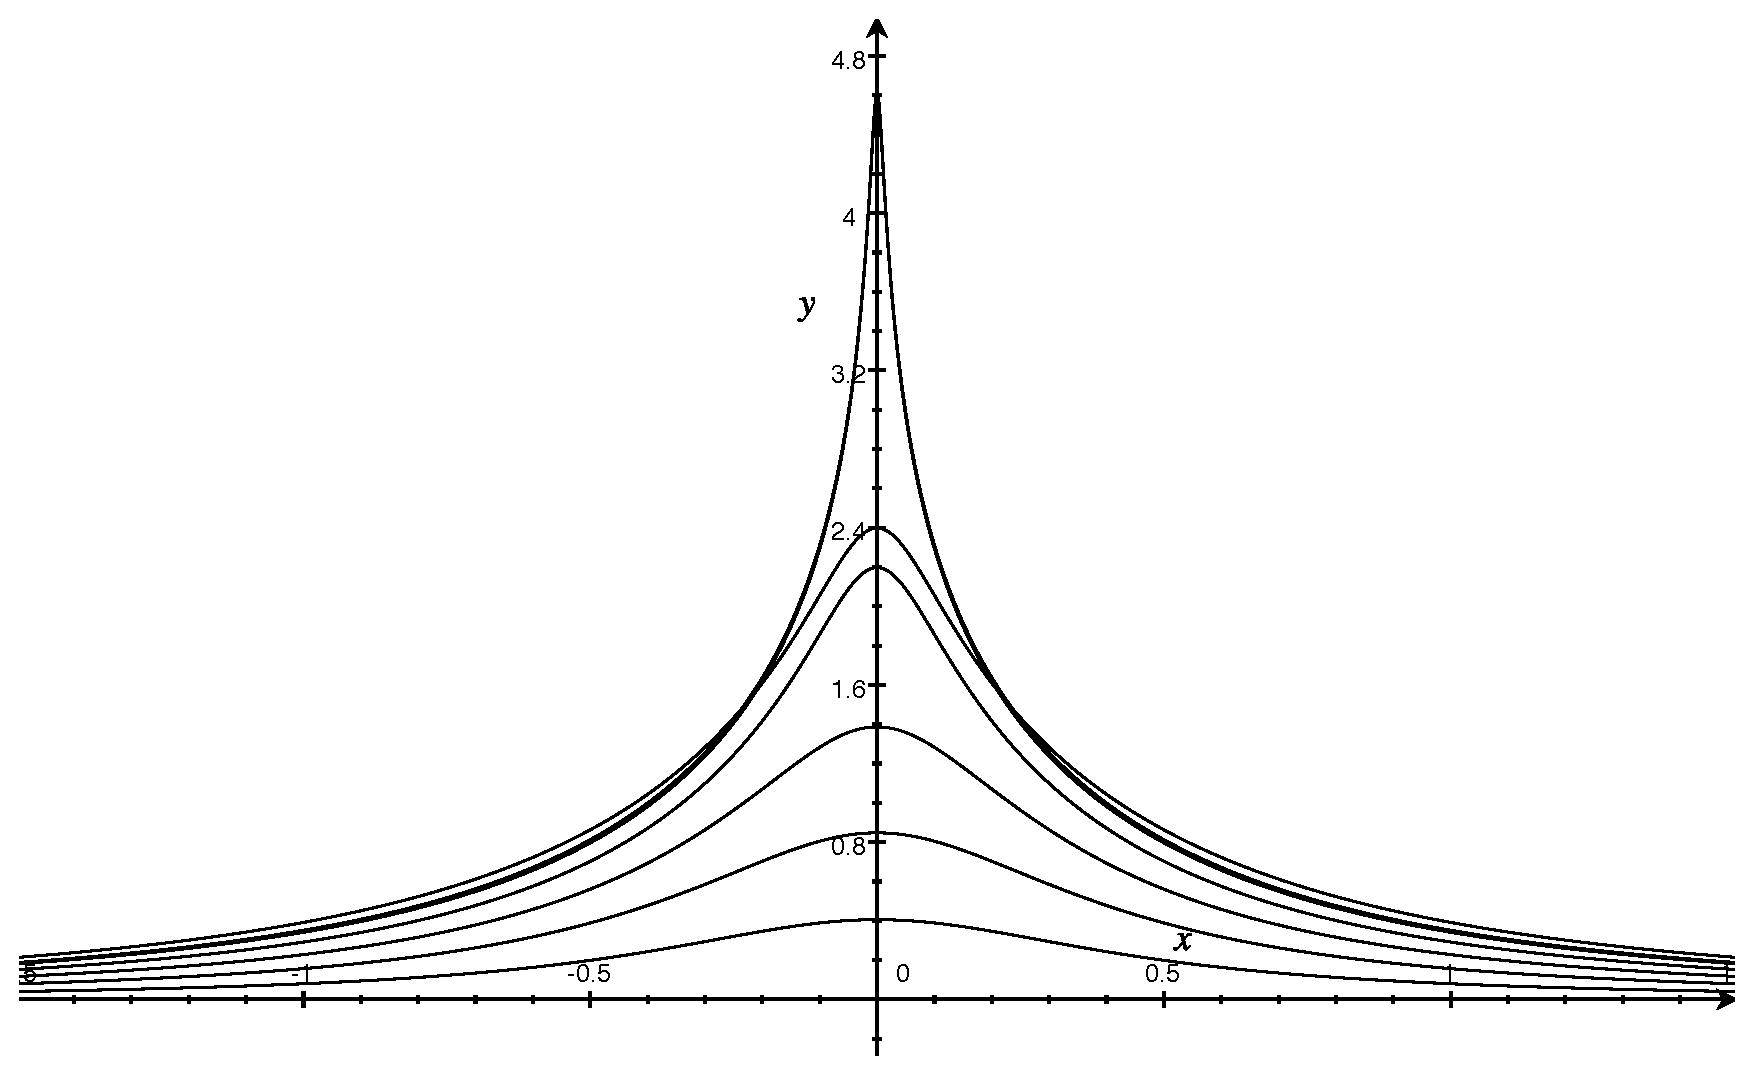
\includegraphics[width=0.48\linewidth]{Figs/Grapher/ModelGreen/reg.eps}
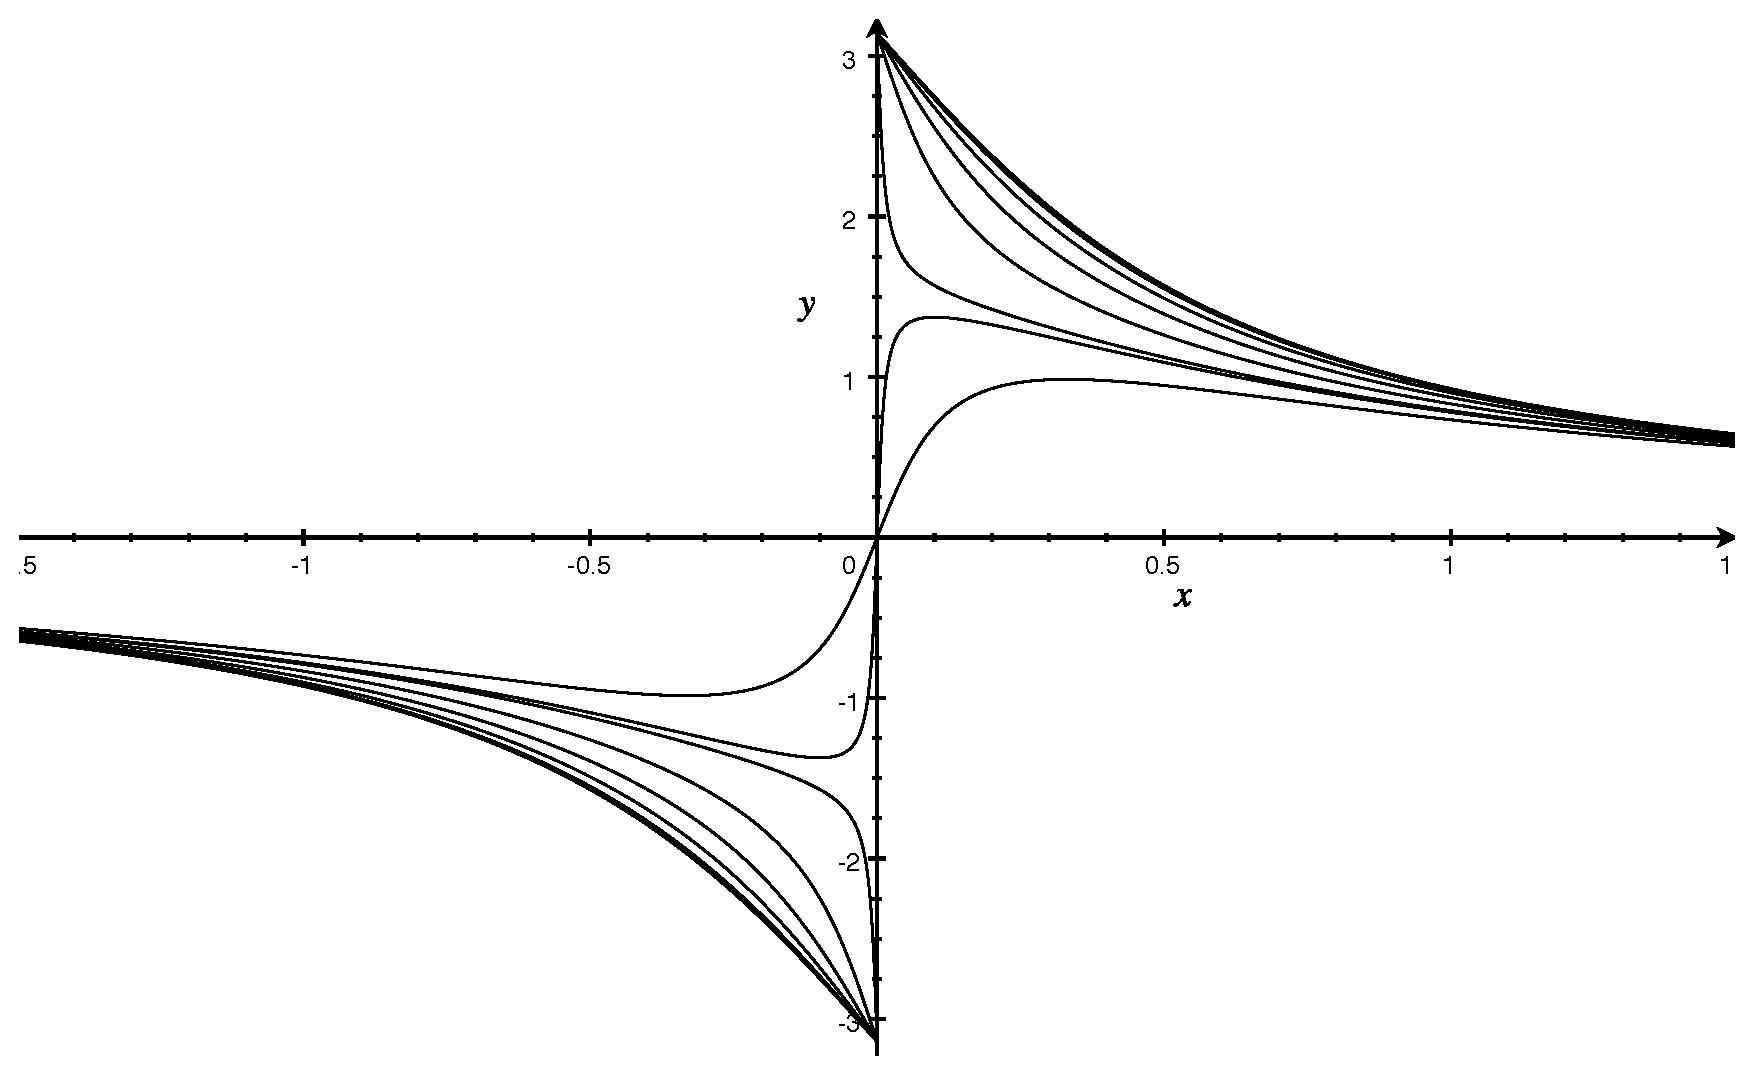
\includegraphics[width=0.48\linewidth]{Figs/Grapher/ModelGreen/img.eps}
\end{center}
\caption{\label{fig:modelgreen}Negative real part (left) and negative imaginary
  part (right) of the Greens function with a constant density of
  states of width $W=1$, centered at
  $E=\{0,0.1,0.2,0.3,0.49,0.51,0.6\}$.}
\end{figure}
The real part is symmetric about
the origin, while the imaginary part is antisymmetric. This is
consistent with $\mat{G}(-i\omega_\nu)=\mat{G}^\dagger(-i\omega_\nu)$.

The imaginary part exhibits a
step at the origin from $\pi/W$ to $\pi/W$ for metallic systems, that is
for a finite density of states at the origin.  For an insulating
system the imaginary part of the Green's function is smooth and has a
finite slope at the origin. 

The real part is positive if the band is
centered above the chemical potential and it is negative if it is
centered below. The real part vanishes if the density of states at the
Fermi level. The real part becomes spiky exactly when the band
touches the Fermi level. As the density of states shifts further to
positive energies, the Greens function grows further in the tails, but
it shrinks in the central region.


\petertt{The following is not correct! Please check!}

Limiting cases
\begin{itemize}
\item $\hbar\omega\rightarrow 0$:

We use the expansion of the arcus tangens
\footnote{
\begin{eqnarray}
  atan(x)&=&y\quad\Rightarrow\quad y=tan(x)=\frac{\sin(x)}{\cos(x)}
\nonumber\\
x&=&\frac{1}{\frac{\pi}{2}-y}+O(y-\frac{\pi}{2})^2
\quad\Rightarrow\quad 
y\approx\frac{\pi}{2}-\frac{1}{x}\quad\text{for $x\rightarrow+\infty$}
\nonumber\\
x&=&\frac{1}{y+\frac{\pi}{2}}+O(y+\frac{\pi}{2})^2
\quad\Rightarrow\quad 
y\approx-\frac{\pi}{2}+\frac{1}{x}\quad\text{for $x\rightarrow-\infty$}
\end{eqnarray}
} and the expanion of the logarithm
\footnote{
\begin{eqnarray}
\ln\left[\frac{a+x}{b+x}\right]\approx
\ln\left[\frac{a}{b}\right]+\left(\frac{1}{a}+\frac{1}{b}\right)x+O(x^2)
\end{eqnarray}
}.
\begin{eqnarray}
G_{a,b}(i\omega_\nu)&=&
\frac{\delta_{a,b}}{W}
\biggl\lbrace
+\frac{1}{2}\ln\left[
\frac{(\hbar\omega)^2+(E-W/2)^2}{(\hbar\omega)^2+(E+W/2)^2}
\right]
-i \left[\atan\left(\frac{E+W/2}{\hbar\omega}\right)
-\atan\left(\frac{E-W/2}{\hbar\omega}\right)\right]
\biggr\rbrace
\nonumber\\
%
&\approx&
\frac{\delta_{a,b}}{W}
\biggl\lbrace
+\frac{1}{2}\ln\left[\left(
\frac{(E-W/2)}{(E+W/2)}\right)^2
\right]
+\frac{1}{2}\left[\frac{1}{(E-W/2)^2}-\frac{1}{(E+W/2)^2}\right]\hbar\omega^2
\nonumber\\
&&-i \left[\frac{\pi}{2}-\frac{\hbar\omega}{E+W/2}
\underbrace{
-\frac{\pi}{2}+\frac{\hbar\omega}{E-W/2}
}_{\text{times -1 for insulators}}\right]
\biggr\rbrace
\nonumber\\
%
&\approx&
\frac{\delta_{a,b}}{W}
\biggl\lbrace
+\ln\left[
\frac{(E-W/2)}{(E+W/2)}
\right]
+\frac{EW}{\left(E^2-\left(\frac{W}{2}\right)^2\right)^2}\hbar\omega^2
-i 
\begin{cases}
\frac{W}{E^2-\left(\frac{W}{2}\right)^2}\hbar\omega
&\text{for insulators}\\
\pm\pi-\frac{4|E|}{E^2-\left(\frac{W}{2}\right)^2}\hbar\omega
&\text{for metals}\\
\end{cases}
\hspace{0.3cm}\biggr\rbrace
\nonumber\\
\end{eqnarray}
%
\item $\hbar\omega\rightarrow \infty$:
\begin{eqnarray}
G_{a,b}(i\omega_\nu)&=&
\frac{\delta_{a,b}}{W}
\biggl\lbrace
+\frac{1}{2}\ln\left[
\frac{(\hbar\omega)^2+(E-W/2)^2}{(\hbar\omega)^2+(E+W/2)^2}
\right]
-i \left[\atan\left(\frac{E+W/2}{\hbar\omega}\right)
-\atan\left(\frac{E-W/2}{\hbar\omega}\right)\right]
\biggr\rbrace
\nonumber\\
%
&\approx&
\frac{\delta_{a,b}}{W}
\biggl\lbrace
-EW(\hbar\omega)^{-2}
-i W (\hbar\omega)^{-1}
\biggr\rbrace
%
\nonumber\\
&\approx&
\delta_{a,b}
\biggl\lbrace
-E(\hbar\omega)^{-2}
-i  (\hbar\omega)^{-1}
\biggr\rbrace
\end{eqnarray}
\end{itemize}


Remark: We can approximate
\begin{eqnarray}
\frac{1}{G_{a,a}^2}\approx \left(
\frac{1}{W}\ln\left[\frac{E-W/2}{E+W/2}\right] \right)^{-2}
  +(\hbar\omega)^2
\end{eqnarray}






%==============================================================================
\section{Bloch representation}
%==============================================================================



\clearpage
\bibliographystyle{unsrtnat} 
 \bibliography{../all}
\end{document}  
 
